\documentclass[11pt, a4paper]{report}

%%%%%%%%%%%%%%%%%%%%%%%%%%%%%%%%%
% PACKAGE IMPORTS
%%%%%%%%%%%%%%%%%%%%%%%%%%%%%%%%%


\usepackage[tmargin=2cm,rmargin=1in,lmargin=1in,margin=0.85in,bmargin=2cm,footskip=.2in]{geometry}
\usepackage{amsmath,amsfonts,amsthm,amssymb,mathtools}
\usepackage[varbb]{newpxmath}
\usepackage{xfrac}
\usepackage[makeroom]{cancel}
\usepackage{mathtools}
\usepackage{bookmark}
\usepackage{enumitem}
\usepackage{subcaption}
% \usepackage{physics}
\usepackage{hyperref,theoremref}
\hypersetup{
	pdftitle={Assignment},
	colorlinks=true, linkcolor=doc!90,
	bookmarksnumbered=true,
	bookmarksopen=true
}
\usepackage[most,many,breakable]{tcolorbox}
\usepackage{xcolor}
\usepackage{varwidth}
\usepackage{varwidth}
\usepackage{etoolbox}
%\usepackage{authblk}
\usepackage{nameref}
\usepackage{multicol,array}
\usepackage{tikz-cd}
\usepackage[ruled,vlined,linesnumbered]{algorithm2e}
\usepackage{comment} % enables the use of multi-line comments (\ifx \fi) 
\usepackage{import}
\usepackage{xifthen}
\usepackage{pdfpages}
\usepackage{transparent}

\newcommand\mycommfont[1]{\footnotesize\ttfamily\textcolor{blue}{#1}}
\SetCommentSty{mycommfont}
\newcommand{\incfig}[1]{%
    \def\svgwidth{\columnwidth}
    \import{./figures/}{#1.pdf_tex}
}

\usepackage{tikzsymbols}
\renewcommand\qedsymbol{$\Laughey$}


%\usepackage{import}
%\usepackage{xifthen}
%\usepackage{pdfpages}
%\usepackage{transparent}


%%%%%%%%%%%%%%%%%%%%%%%%%%%%%%
% SELF MADE COLORS
%%%%%%%%%%%%%%%%%%%%%%%%%%%%%%



\definecolor{myg}{RGB}{56, 140, 70}
\definecolor{myb}{RGB}{45, 111, 177}
\definecolor{myr}{RGB}{199, 68, 64}
\definecolor{mytheorembg}{HTML}{F2F2F9}
\definecolor{mytheoremfr}{HTML}{00007B}
\definecolor{mylenmabg}{HTML}{FFFAF8}
\definecolor{mylenmafr}{HTML}{983b0f}
\definecolor{mypropbg}{HTML}{f2fbfc}
\definecolor{mypropfr}{HTML}{191971}
\definecolor{myexamplebg}{HTML}{F2FBF8}
\definecolor{myexamplefr}{HTML}{88D6D1}
\definecolor{myexampleti}{HTML}{2A7F7F}
\definecolor{mydefinitbg}{HTML}{E5E5FF}
\definecolor{mydefinitfr}{HTML}{3F3FA3}
\definecolor{notesgreen}{RGB}{0,162,0}
\definecolor{myp}{RGB}{197, 92, 212}
\definecolor{mygr}{HTML}{2C3338}
\definecolor{myred}{RGB}{127,0,0}
\definecolor{myyellow}{RGB}{169,121,69}
\definecolor{myexercisebg}{HTML}{F2FBF8}
\definecolor{myexercisefg}{HTML}{88D6D1}


%%%%%%%%%%%%%%%%%%%%%%%%%%%%
% TCOLORBOX SETUPS
%%%%%%%%%%%%%%%%%%%%%%%%%%%%

\setlength{\parindent}{1cm}
%================================
% THEOREM BOX
%================================

\tcbuselibrary{theorems,skins,hooks}
\newtcbtheorem[number within=section]{Theorem}{Theorem}
{%
	enhanced,
	breakable,
	colback = mytheorembg,
	frame hidden,
	boxrule = 0sp,
	borderline west = {2pt}{0pt}{mytheoremfr},
	sharp corners,
	detach title,
	before upper = \tcbtitle\par\smallskip,
	coltitle = mytheoremfr,
	fonttitle = \bfseries\sffamily,
	description font = \mdseries,
	separator sign none,
	segmentation style={solid, mytheoremfr},
}
{th}

\tcbuselibrary{theorems,skins,hooks}
\newtcbtheorem[number within=chapter]{theorem}{Theorem}
{%
	enhanced,
	breakable,
	colback = mytheorembg,
	frame hidden,
	boxrule = 0sp,
	borderline west = {2pt}{0pt}{mytheoremfr},
	sharp corners,
	detach title,
	before upper = \tcbtitle\par\smallskip,
	coltitle = mytheoremfr,
	fonttitle = \bfseries\sffamily,
	description font = \mdseries,
	separator sign none,
	segmentation style={solid, mytheoremfr},
}
{th}


\tcbuselibrary{theorems,skins,hooks}
\newtcolorbox{Theoremcon}
{%
	enhanced
	,breakable
	,colback = mytheorembg
	,frame hidden
	,boxrule = 0sp
	,borderline west = {2pt}{0pt}{mytheoremfr}
	,sharp corners
	,description font = \mdseries
	,separator sign none
}

%================================
% Corollery
%================================
\tcbuselibrary{theorems,skins,hooks}
\newtcbtheorem[number within=section]{Corollary}{Corollary}
{%
	enhanced
	,breakable
	,colback = myp!10
	,frame hidden
	,boxrule = 0sp
	,borderline west = {2pt}{0pt}{myp!85!black}
	,sharp corners
	,detach title
	,before upper = \tcbtitle\par\smallskip
	,coltitle = myp!85!black
	,fonttitle = \bfseries\sffamily
	,description font = \mdseries
	,separator sign none
	,segmentation style={solid, myp!85!black}
}
{th}
\tcbuselibrary{theorems,skins,hooks}
\newtcbtheorem[number within=chapter]{corollary}{Corollary}
{%
	enhanced
	,breakable
	,colback = myp!10
	,frame hidden
	,boxrule = 0sp
	,borderline west = {2pt}{0pt}{myp!85!black}
	,sharp corners
	,detach title
	,before upper = \tcbtitle\par\smallskip
	,coltitle = myp!85!black
	,fonttitle = \bfseries\sffamily
	,description font = \mdseries
	,separator sign none
	,segmentation style={solid, myp!85!black}
}
{th}


%================================
% LENMA
%================================

\tcbuselibrary{theorems,skins,hooks}
\newtcbtheorem[number within=section]{Lenma}{Lenma}
{%
	enhanced,
	breakable,
	colback = mylenmabg,
	frame hidden,
	boxrule = 0sp,
	borderline west = {2pt}{0pt}{mylenmafr},
	sharp corners,
	detach title,
	before upper = \tcbtitle\par\smallskip,
	coltitle = mylenmafr,
	fonttitle = \bfseries\sffamily,
	description font = \mdseries,
	separator sign none,
	segmentation style={solid, mylenmafr},
}
{th}

\tcbuselibrary{theorems,skins,hooks}
\newtcbtheorem[number within=chapter]{lenma}{Lenma}
{%
	enhanced,
	breakable,
	colback = mylenmabg,
	frame hidden,
	boxrule = 0sp,
	borderline west = {2pt}{0pt}{mylenmafr},
	sharp corners,
	detach title,
	before upper = \tcbtitle\par\smallskip,
	coltitle = mylenmafr,
	fonttitle = \bfseries\sffamily,
	description font = \mdseries,
	separator sign none,
	segmentation style={solid, mylenmafr},
}
{th}


%================================
% PROPOSITION
%================================

\tcbuselibrary{theorems,skins,hooks}
\newtcbtheorem[number within=section]{Prop}{Proposition}
{%
	enhanced,
	breakable,
	colback = mypropbg,
	frame hidden,
	boxrule = 0sp,
	borderline west = {2pt}{0pt}{mypropfr},
	sharp corners,
	detach title,
	before upper = \tcbtitle\par\smallskip,
	coltitle = mypropfr,
	fonttitle = \bfseries\sffamily,
	description font = \mdseries,
	separator sign none,
	segmentation style={solid, mypropfr},
}
{th}

\tcbuselibrary{theorems,skins,hooks}
\newtcbtheorem[number within=chapter]{prop}{Proposition}
{%
	enhanced,
	breakable,
	colback = mypropbg,
	frame hidden,
	boxrule = 0sp,
	borderline west = {2pt}{0pt}{mypropfr},
	sharp corners,
	detach title,
	before upper = \tcbtitle\par\smallskip,
	coltitle = mypropfr,
	fonttitle = \bfseries\sffamily,
	description font = \mdseries,
	separator sign none,
	segmentation style={solid, mypropfr},
}
{th}


%================================
% CLAIM
%================================

\tcbuselibrary{theorems,skins,hooks}
\newtcbtheorem[number within=section]{claim}{Claim}
{%
	enhanced
	,breakable
	,colback = myg!10
	,frame hidden
	,boxrule = 0sp
	,borderline west = {2pt}{0pt}{myg}
	,sharp corners
	,detach title
	,before upper = \tcbtitle\par\smallskip
	,coltitle = myg!85!black
	,fonttitle = \bfseries\sffamily
	,description font = \mdseries
	,separator sign none
	,segmentation style={solid, myg!85!black}
}
{th}



%================================
% Exercise
%================================

\tcbuselibrary{theorems,skins,hooks}
\newtcbtheorem[number within=section]{Exercise}{Exercise}
{%
	enhanced,
	breakable,
	colback = myexercisebg,
	frame hidden,
	boxrule = 0sp,
	borderline west = {2pt}{0pt}{myexercisefg},
	sharp corners,
	detach title,
	before upper = \tcbtitle\par\smallskip,
	coltitle = myexercisefg,
	fonttitle = \bfseries\sffamily,
	description font = \mdseries,
	separator sign none,
	segmentation style={solid, myexercisefg},
}
{th}

\tcbuselibrary{theorems,skins,hooks}
\newtcbtheorem[number within=chapter]{exercise}{Exercise}
{%
	enhanced,
	breakable,
	colback = myexercisebg,
	frame hidden,
	boxrule = 0sp,
	borderline west = {2pt}{0pt}{myexercisefg},
	sharp corners,
	detach title,
	before upper = \tcbtitle\par\smallskip,
	coltitle = myexercisefg,
	fonttitle = \bfseries\sffamily,
	description font = \mdseries,
	separator sign none,
	segmentation style={solid, myexercisefg},
}
{th}

%================================
% EXAMPLE BOX
%================================

\newtcbtheorem[number within=section]{Example}{Example}
{%
	colback = myexamplebg
	,breakable
	,colframe = myexamplefr
	,coltitle = myexampleti
	,boxrule = 1pt
	,sharp corners
	,detach title
	,before upper=\tcbtitle\par\smallskip
	,fonttitle = \bfseries
	,description font = \mdseries
	,separator sign none
	,description delimiters parenthesis
}
{ex}

\newtcbtheorem[number within=chapter]{example}{Example}
{%
	colback = myexamplebg
	,breakable
	,colframe = myexamplefr
	,coltitle = myexampleti
	,boxrule = 1pt
	,sharp corners
	,detach title
	,before upper=\tcbtitle\par\smallskip
	,fonttitle = \bfseries
	,description font = \mdseries
	,separator sign none
	,description delimiters parenthesis
}
{ex}

%================================
% DEFINITION BOX
%================================

\newtcbtheorem[number within=section]{Definition}{Definition}{enhanced,
	before skip=2mm,after skip=2mm, colback=red!5,colframe=red!80!black,boxrule=0.5mm,
	attach boxed title to top left={xshift=1cm,yshift*=1mm-\tcboxedtitleheight}, varwidth boxed title*=-3cm,
	boxed title style={frame code={
					\path[fill=tcbcolback]
					([yshift=-1mm,xshift=-1mm]frame.north west)
					arc[start angle=0,end angle=180,radius=1mm]
					([yshift=-1mm,xshift=1mm]frame.north east)
					arc[start angle=180,end angle=0,radius=1mm];
					\path[left color=tcbcolback!60!black,right color=tcbcolback!60!black,
						middle color=tcbcolback!80!black]
					([xshift=-2mm]frame.north west) -- ([xshift=2mm]frame.north east)
					[rounded corners=1mm]-- ([xshift=1mm,yshift=-1mm]frame.north east)
					-- (frame.south east) -- (frame.south west)
					-- ([xshift=-1mm,yshift=-1mm]frame.north west)
					[sharp corners]-- cycle;
				},interior engine=empty,
		},
	fonttitle=\bfseries,
	title={#2},#1}{def}
\newtcbtheorem[number within=chapter]{definition}{Definition}{enhanced,
	before skip=2mm,after skip=2mm, colback=red!5,colframe=red!80!black,boxrule=0.5mm,
	attach boxed title to top left={xshift=1cm,yshift*=1mm-\tcboxedtitleheight}, varwidth boxed title*=-3cm,
	boxed title style={frame code={
					\path[fill=tcbcolback]
					([yshift=-1mm,xshift=-1mm]frame.north west)
					arc[start angle=0,end angle=180,radius=1mm]
					([yshift=-1mm,xshift=1mm]frame.north east)
					arc[start angle=180,end angle=0,radius=1mm];
					\path[left color=tcbcolback!60!black,right color=tcbcolback!60!black,
						middle color=tcbcolback!80!black]
					([xshift=-2mm]frame.north west) -- ([xshift=2mm]frame.north east)
					[rounded corners=1mm]-- ([xshift=1mm,yshift=-1mm]frame.north east)
					-- (frame.south east) -- (frame.south west)
					-- ([xshift=-1mm,yshift=-1mm]frame.north west)
					[sharp corners]-- cycle;
				},interior engine=empty,
		},
	fonttitle=\bfseries,
	title={#2},#1}{def}



%================================
% Solution BOX
%================================

\makeatletter
\newtcbtheorem{question}{Question}{enhanced,
	breakable,
	colback=white,
	colframe=myb!80!black,
	attach boxed title to top left={yshift*=-\tcboxedtitleheight},
	fonttitle=\bfseries,
	title={#2},
	boxed title size=title,
	boxed title style={%
			sharp corners,
			rounded corners=northwest,
			colback=tcbcolframe,
			boxrule=0pt,
		},
	underlay boxed title={%
			\path[fill=tcbcolframe] (title.south west)--(title.south east)
			to[out=0, in=180] ([xshift=5mm]title.east)--
			(title.center-|frame.east)
			[rounded corners=\kvtcb@arc] |-
			(frame.north) -| cycle;
		},
	#1
}{def}
\makeatother

%================================
% SOLUTION BOX
%================================

\makeatletter
\newtcolorbox{solution}{enhanced,
	breakable,
	colback=white,
	colframe=myg!80!black,
	attach boxed title to top left={yshift*=-\tcboxedtitleheight},
	title=Solution,
	boxed title size=title,
	boxed title style={%
			sharp corners,
			rounded corners=northwest,
			colback=tcbcolframe,
			boxrule=0pt,
		},
	underlay boxed title={%
			\path[fill=tcbcolframe] (title.south west)--(title.south east)
			to[out=0, in=180] ([xshift=5mm]title.east)--
			(title.center-|frame.east)
			[rounded corners=\kvtcb@arc] |-
			(frame.north) -| cycle;
		},
}
\makeatother

%================================
% Question BOX
%================================

\makeatletter
\newtcbtheorem{qstion}{Question}{enhanced,
	breakable,
	colback=white,
	colframe=mygr,
	attach boxed title to top left={yshift*=-\tcboxedtitleheight},
	fonttitle=\bfseries,
	title={#2},
	boxed title size=title,
	boxed title style={%
			sharp corners,
			rounded corners=northwest,
			colback=tcbcolframe,
			boxrule=0pt,
		},
	underlay boxed title={%
			\path[fill=tcbcolframe] (title.south west)--(title.south east)
			to[out=0, in=180] ([xshift=5mm]title.east)--
			(title.center-|frame.east)
			[rounded corners=\kvtcb@arc] |-
			(frame.north) -| cycle;
		},
	#1
}{def}
\makeatother

\newtcbtheorem[number within=chapter]{wconc}{Wrong Concept}{
	breakable,
	enhanced,
	colback=white,
	colframe=myr,
	arc=0pt,
	outer arc=0pt,
	fonttitle=\bfseries\sffamily\large,
	colbacktitle=myr,
	attach boxed title to top left={},
	boxed title style={
			enhanced,
			skin=enhancedfirst jigsaw,
			arc=3pt,
			bottom=0pt,
			interior style={fill=myr}
		},
	#1
}{def}



%================================
% NOTE BOX
%================================

\usetikzlibrary{arrows,calc,shadows.blur}
\tcbuselibrary{skins}
\newtcolorbox{note}[1][]{%
	enhanced jigsaw,
	colback=gray!20!white,%
	colframe=gray!80!black,
	size=small,
	boxrule=1pt,
	title=\textbf{Note:-},
	halign title=flush center,
	coltitle=black,
	breakable,
	drop shadow=black!50!white,
	attach boxed title to top left={xshift=1cm,yshift=-\tcboxedtitleheight/2,yshifttext=-\tcboxedtitleheight/2},
	minipage boxed title=1.5cm,
	boxed title style={%
			colback=white,
			size=fbox,
			boxrule=1pt,
			boxsep=2pt,
			underlay={%
					\coordinate (dotA) at ($(interior.west) + (-0.5pt,0)$);
					\coordinate (dotB) at ($(interior.east) + (0.5pt,0)$);
					\begin{scope}
						\clip (interior.north west) rectangle ([xshift=3ex]interior.east);
						\filldraw [white, blur shadow={shadow opacity=60, shadow yshift=-.75ex}, rounded corners=2pt] (interior.north west) rectangle (interior.south east);
					\end{scope}
					\begin{scope}[gray!80!black]
						\fill (dotA) circle (2pt);
						\fill (dotB) circle (2pt);
					\end{scope}
				},
		},
	#1,
}

%%%%%%%%%%%%%%%%%%%%%%%%%%%%%%
% SELF MADE COMMANDS
%%%%%%%%%%%%%%%%%%%%%%%%%%%%%%


\newcommand{\thm}[2]{\begin{Theorem}{#1}{}#2\end{Theorem}}
\newcommand{\cor}[2]{\begin{Corollary}{#1}{}#2\end{Corollary}}
\newcommand{\mlenma}[2]{\begin{Lenma}{#1}{}#2\end{Lenma}}
\newcommand{\mprop}[2]{\begin{Prop}{#1}{}#2\end{Prop}}
\newcommand{\clm}[3]{\begin{claim}{#1}{#2}#3\end{claim}}
\newcommand{\wc}[2]{\begin{wconc}{#1}{}\setlength{\parindent}{1cm}#2\end{wconc}}
\newcommand{\thmcon}[1]{\begin{Theoremcon}{#1}\end{Theoremcon}}
\newcommand{\ex}[2]{\begin{Example}{#1}{}#2\end{Example}}
\newcommand{\dfn}[2]{\begin{Definition}[colbacktitle=red!75!black]{#1}{}#2\end{Definition}}
\newcommand{\dfnc}[2]{\begin{definition}[colbacktitle=red!75!black]{#1}{}#2\end{definition}}
\newcommand{\qs}[2]{\begin{question}{#1}{}#2\end{question}}
\newcommand{\pf}[2]{\begin{myproof}[#1]#2\end{myproof}}
\newcommand{\nt}[1]{\begin{note}#1\end{note}}

\newcommand*\circled[1]{\tikz[baseline=(char.base)]{
		\node[shape=circle,draw,inner sep=1pt] (char) {#1};}}
\newcommand\getcurrentref[1]{%
	\ifnumequal{\value{#1}}{0}
	{??}
	{\the\value{#1}}%
}
\newcommand{\getCurrentSectionNumber}{\getcurrentref{section}}
\newenvironment{myproof}[1][\proofname]{%
	\proof[\bfseries #1: ]%
}{\endproof}

\newcommand{\mclm}[2]{\begin{myclaim}[#1]#2\end{myclaim}}
\newenvironment{myclaim}[1][\claimname]{\proof[\bfseries #1: ]}{}

\newcounter{mylabelcounter}

\makeatletter
\newcommand{\setword}[2]{%
	\phantomsection
	#1\def\@currentlabel{\unexpanded{#1}}\label{#2}%
}
\makeatother




\tikzset{
	symbol/.style={
			draw=none,
			every to/.append style={
					edge node={node [sloped, allow upside down, auto=false]{$#1$}}}
		}
}


% deliminators
\DeclarePairedDelimiter{\abs}{\lvert}{\rvert}
\DeclarePairedDelimiter{\norm}{\lVert}{\rVert}

\DeclarePairedDelimiter{\ceil}{\lceil}{\rceil}
\DeclarePairedDelimiter{\floor}{\lfloor}{\rfloor}
\DeclarePairedDelimiter{\round}{\lfloor}{\rceil}

\newsavebox\diffdbox
\newcommand{\slantedromand}{{\mathpalette\makesl{d}}}
\newcommand{\makesl}[2]{%
\begingroup
\sbox{\diffdbox}{$\mathsurround=0pt#1\mathrm{#2}$}%
\pdfsave
\pdfsetmatrix{1 0 0.2 1}%
\rlap{\usebox{\diffdbox}}%
\pdfrestore
\hskip\wd\diffdbox
\endgroup
}
\newcommand{\dd}[1][]{\ensuremath{\mathop{}\!\ifstrempty{#1}{%
\slantedromand\@ifnextchar^{\hspace{0.2ex}}{\hspace{0.1ex}}}%
{\slantedromand\hspace{0.2ex}^{#1}}}}
\ProvideDocumentCommand\dv{o m g}{%
  \ensuremath{%
    \IfValueTF{#3}{%
      \IfNoValueTF{#1}{%
        \frac{\dd #2}{\dd #3}%
      }{%
        \frac{\dd^{#1} #2}{\dd #3^{#1}}%
      }%
    }{%
      \IfNoValueTF{#1}{%
        \frac{\dd}{\dd #2}%
      }{%
        \frac{\dd^{#1}}{\dd #2^{#1}}%
      }%
    }%
  }%
}
\providecommand*{\pdv}[3][]{\frac{\partial^{#1}#2}{\partial#3^{#1}}}
%  - others
\DeclareMathOperator{\Lap}{\mathcal{L}}
\DeclareMathOperator{\Var}{Var} % varience
\DeclareMathOperator{\Cov}{Cov} % covarience
\DeclareMathOperator{\E}{E} % expected

% Since the amsthm package isn't loaded

% I prefer the slanted \leq
\let\oldleq\leq % save them in case they're every wanted
\let\oldgeq\geq
\renewcommand{\leq}{\leqslant}
\renewcommand{\geq}{\geqslant}

% % redefine matrix env to allow for alignment, use r as default
% \renewcommand*\env@matrix[1][r]{\hskip -\arraycolsep
%     \let\@ifnextchar\new@ifnextchar
%     \array{*\c@MaxMatrixCols #1}}


%\usepackage{framed}
%\usepackage{titletoc}
%\usepackage{etoolbox}
%\usepackage{lmodern}


%\patchcmd{\tableofcontents}{\contentsname}{\sffamily\contentsname}{}{}

%\renewenvironment{leftbar}
%{\def\FrameCommand{\hspace{6em}%
%		{\color{myyellow}\vrule width 2pt depth 6pt}\hspace{1em}}%
%	\MakeFramed{\parshape 1 0cm \dimexpr\textwidth-6em\relax\FrameRestore}\vskip2pt%
%}
%{\endMakeFramed}

%\titlecontents{chapter}
%[0em]{\vspace*{2\baselineskip}}
%{\parbox{4.5em}{%
%		\hfill\Huge\sffamily\bfseries\color{myred}\thecontentspage}%
%	\vspace*{-2.3\baselineskip}\leftbar\textsc{\small\chaptername~\thecontentslabel}\\\sffamily}
%{}{\endleftbar}
%\titlecontents{section}
%[8.4em]
%{\sffamily\contentslabel{3em}}{}{}
%{\hspace{0.5em}\nobreak\itshape\color{myred}\contentspage}
%\titlecontents{subsection}
%[8.4em]
%{\sffamily\contentslabel{3em}}{}{}  
%{\hspace{0.5em}\nobreak\itshape\color{myred}\contentspage}



%%%%%%%%%%%%%%%%%%%%%%%%%%%%%%%%%%%%%%%%%%%
% TABLE OF CONTENTS
%%%%%%%%%%%%%%%%%%%%%%%%%%%%%%%%%%%%%%%%%%%

\usepackage{tikz}
\definecolor{doc}{RGB}{0,60,110}
\usepackage{titletoc}
\contentsmargin{0cm}
\titlecontents{chapter}[3.7pc]
{\addvspace{30pt}%
	\begin{tikzpicture}[remember picture, overlay]%
		\draw[fill=doc!60,draw=doc!60] (-7,-.1) rectangle (-0.9,.5);%
		\pgftext[left,x=-3.5cm,y=0.2cm]{\color{white}\Large\sc\bfseries Chapter\ \thecontentslabel};%
	\end{tikzpicture}\color{doc!60}\large\sc\bfseries}%
{}
{}
{\;\titlerule\;\large\sc\bfseries Page \thecontentspage
	\begin{tikzpicture}[remember picture, overlay]
		\draw[fill=doc!60,draw=doc!60] (2pt,0) rectangle (4,0.1pt);
	\end{tikzpicture}}%
\titlecontents{section}[3.7pc]
{\addvspace{2pt}}
{\contentslabel[\thecontentslabel]{2pc}}
{}
{\hfill\small \thecontentspage}
[]
\titlecontents*{subsection}[3.7pc]
{\addvspace{-1pt}\small}
{}
{}
{\ --- \small\thecontentspage}
[ \textbullet\ ][]

\makeatletter
\renewcommand{\tableofcontents}{%
	\chapter*{%
	  \vspace*{-20\p@}%
	  \begin{tikzpicture}[remember picture, overlay]%
		  \pgftext[right,x=15cm,y=0.2cm]{\color{doc!60}\Huge\sc\bfseries \contentsname};%
		  \draw[fill=doc!60,draw=doc!60] (13,-.75) rectangle (20,1);%
		  \clip (13,-.75) rectangle (20,1);
		  \pgftext[right,x=15cm,y=0.2cm]{\color{white}\Huge\sc\bfseries \contentsname};%
	  \end{tikzpicture}}%
	\@starttoc{toc}}
\makeatother


\usepackage[svgnames]{xcolor} % Required to specify font color

\newcommand*{\plogo}{\fbox{$\mathcal{PL}$}} % Generic publisher logo

\usepackage{graphicx} % Required for box manipulation

%----------------------------------------------------------------------------------------
%	TITLE PAGE
%----------------------------------------------------------------------------------------

\newcommand*{\rotrt}[1]{\rotatebox{90}{#1}} % Command to rotate right 90 degrees
\newcommand*{\rotlft}[1]{\rotatebox{-90}{#1}} % Command to rotate left 90 degrees

\newcommand*{\titleBC}{\begingroup % Create the command for including the title page in the document
\centering % Center all text

\def\CP{\textit{\Huge Queueing Theory - Seminar Notes}} % Title

\settowidth{\unitlength}{\CP} % Set the width of the curly brackets to the width of the title
{\color{LightGoldenrod}\resizebox*{\unitlength}{\baselineskip}{\rotrt{$\}$}}} \\[\baselineskip] % Print top curly bracket
\textcolor{Sienna}{\CP} \\[\baselineskip] % Print title
{\color{RosyBrown}\Large A Mathematically-Rigorous yet Intuitive Introduction to Queues} \\ % Tagline or further description
{\color{LightGoldenrod}\resizebox*{\unitlength}{\baselineskip}{\rotlft{$\}$}}} % Print bottom curly bracket

\vfill % Whitespace between the title and the author name

{\Large\textbf{Rishabh Pomaje}\\ \href{mailto:210020036@iitdh.ac.in}{210020036@iitdh.ac.in}}\\ % Author name

\vfill % Whitespace between the author name and the publisher logo

\endgroup}

%From M275 "Topology" at SJSU
\newcommand{\id}{\mathrm{id}}
\newcommand{\taking}[1]{\xrightarrow{#1}}
\newcommand{\inv}{^{-1}}

%From M170 "Introduction to Graph Theory" at SJSU
\DeclareMathOperator{\diam}{diam}
\DeclareMathOperator{\ord}{ord}
\newcommand{\defeq}{\overset{\mathrm{def}}{=}}

%From the USAMO .tex files
\newcommand{\ts}{\textsuperscript}
\newcommand{\dg}{^\circ}
\newcommand{\ii}{\item}

% % From Math 55 and Math 145 at Harvard
% \newenvironment{subproof}[1][Proof]{%
% \begin{proof}[#1] \renewcommand{\qedsymbol}{$\blacksquare$}}%
% {\end{proof}}

\newcommand{\liff}{\leftrightarrow}
\newcommand{\lthen}{\rightarrow}
\newcommand{\opname}{\operatorname}
\newcommand{\surjto}{\twoheadrightarrow}
\newcommand{\injto}{\hookrightarrow}
\newcommand{\On}{\mathrm{On}} % ordinals
\DeclareMathOperator{\img}{im} % Image
\DeclareMathOperator{\Img}{Im} % Image
\DeclareMathOperator{\coker}{coker} % Cokernel
\DeclareMathOperator{\Coker}{Coker} % Cokernel
\DeclareMathOperator{\Ker}{Ker} % Kernel
\DeclareMathOperator{\rank}{rank}
\DeclareMathOperator{\Spec}{Spec} % spectrum
\DeclareMathOperator{\Tr}{Tr} % trace
\DeclareMathOperator{\pr}{pr} % projection
\DeclareMathOperator{\ext}{ext} % extension
\DeclareMathOperator{\pred}{pred} % predecessor
\DeclareMathOperator{\dom}{dom} % domain
\DeclareMathOperator{\ran}{ran} % range
\DeclareMathOperator{\Hom}{Hom} % homomorphism
\DeclareMathOperator{\Mor}{Mor} % morphisms
\DeclareMathOperator{\End}{End} % endomorphism

\newcommand{\eps}{\epsilon}
\newcommand{\veps}{\varepsilon}
\newcommand{\ol}{\overline}
\newcommand{\ul}{\underline}
\newcommand{\wt}{\widetilde}
\newcommand{\wh}{\widehat}
\newcommand{\vocab}[1]{\textbf{\color{blue} #1}}
\providecommand{\half}{\frac{1}{2}}
\newcommand{\dang}{\measuredangle} %% Directed angle
\newcommand{\ray}[1]{\overrightarrow{#1}}
\newcommand{\seg}[1]{\overline{#1}}
\newcommand{\arc}[1]{\wideparen{#1}}
\DeclareMathOperator{\cis}{cis}
\DeclareMathOperator*{\lcm}{lcm}
\DeclareMathOperator*{\argmin}{arg min}
\DeclareMathOperator*{\argmax}{arg max}
\newcommand{\cycsum}{\sum_{\mathrm{cyc}}}
\newcommand{\symsum}{\sum_{\mathrm{sym}}}
\newcommand{\cycprod}{\prod_{\mathrm{cyc}}}
\newcommand{\symprod}{\prod_{\mathrm{sym}}}
\newcommand{\Qed}{\begin{flushright}\qed\end{flushright}}
\newcommand{\parinn}{\setlength{\parindent}{1cm}}
\newcommand{\parinf}{\setlength{\parindent}{0cm}}
% \newcommand{\norm}{\|\cdot\|}
\newcommand{\inorm}{\norm_{\infty}}
\newcommand{\opensets}{\{V_{\alpha}\}_{\alpha\in I}}
\newcommand{\oset}{V_{\alpha}}
\newcommand{\opset}[1]{V_{\alpha_{#1}}}
\newcommand{\lub}{\text{lub}}
\newcommand{\del}[2]{\frac{\partial #1}{\partial #2}}
\newcommand{\Del}[3]{\frac{\partial^{#1} #2}{\partial^{#1} #3}}
\newcommand{\deld}[2]{\dfrac{\partial #1}{\partial #2}}
\newcommand{\Deld}[3]{\dfrac{\partial^{#1} #2}{\partial^{#1} #3}}
\newcommand{\lm}{\lambda}
\newcommand{\uin}{\mathbin{\rotatebox[origin=c]{90}{$\in$}}}
\newcommand{\usubset}{\mathbin{\rotatebox[origin=c]{90}{$\subset$}}}
\newcommand{\lt}{\left}
\newcommand{\rt}{\right}
\newcommand{\bs}[1]{\boldsymbol{#1}}
\newcommand{\exs}{\exists}
\newcommand{\st}{\strut}
\newcommand{\dps}[1]{\displaystyle{#1}}

\newcommand{\sol}{\setlength{\parindent}{0cm}\textbf{\textit{Solution:}}\setlength{\parindent}{1cm} }
\newcommand{\solve}[1]{\setlength{\parindent}{0cm}\textbf{\textit{Solution: }}\setlength{\parindent}{1cm}#1 \Qed}

%%%%% NEW MATH DEFINITIONS %%%%%

\usepackage{amsmath,amsfonts,bm}

% Mark sections of captions for referring to divisions of figures
\newcommand{\figleft}{{\em (Left)}}
\newcommand{\figcenter}{{\em (Center)}}
\newcommand{\figright}{{\em (Right)}}
\newcommand{\figtop}{{\em (Top)}}
\newcommand{\figbottom}{{\em (Bottom)}}
\newcommand{\captiona}{{\em (a)}}
\newcommand{\captionb}{{\em (b)}}
\newcommand{\captionc}{{\em (c)}}
\newcommand{\captiond}{{\em (d)}}

% Highlight a newly defined term
\newcommand{\newterm}[1]{{\bf #1}}


% Figure reference, lower-case.
\def\figref#1{figure~\ref{#1}}
% Figure reference, capital. For start of sentence
\def\Figref#1{Figure~\ref{#1}}
\def\twofigref#1#2{figures \ref{#1} and \ref{#2}}
\def\quadfigref#1#2#3#4{figures \ref{#1}, \ref{#2}, \ref{#3} and \ref{#4}}
% Section reference, lower-case.
\def\secref#1{section~\ref{#1}}
% Section reference, capital.
\def\Secref#1{Section~\ref{#1}}
% Reference to two sections.
\def\twosecrefs#1#2{sections \ref{#1} and \ref{#2}}
% Reference to three sections.
\def\secrefs#1#2#3{sections \ref{#1}, \ref{#2} and \ref{#3}}
% Reference to an equation, lower-case.
\def\eqref#1{equation~\ref{#1}}
% Reference to an equation, upper case
\def\Eqref#1{Equation~\ref{#1}}
% A raw reference to an equation---avoid using if possible
\def\plaineqref#1{\ref{#1}}
% Reference to a chapter, lower-case.
\def\chapref#1{chapter~\ref{#1}}
% Reference to an equation, upper case.
\def\Chapref#1{Chapter~\ref{#1}}
% Reference to a range of chapters
\def\rangechapref#1#2{chapters\ref{#1}--\ref{#2}}
% Reference to an algorithm, lower-case.
\def\algref#1{algorithm~\ref{#1}}
% Reference to an algorithm, upper case.
\def\Algref#1{Algorithm~\ref{#1}}
\def\twoalgref#1#2{algorithms \ref{#1} and \ref{#2}}
\def\Twoalgref#1#2{Algorithms \ref{#1} and \ref{#2}}
% Reference to a part, lower case
\def\partref#1{part~\ref{#1}}
% Reference to a part, upper case
\def\Partref#1{Part~\ref{#1}}
\def\twopartref#1#2{parts \ref{#1} and \ref{#2}}

\def\ceil#1{\lceil #1 \rceil}
\def\floor#1{\lfloor #1 \rfloor}
\def\1{\bm{1}}
\newcommand{\train}{\mathcal{D}}
\newcommand{\valid}{\mathcal{D_{\mathrm{valid}}}}
\newcommand{\test}{\mathcal{D_{\mathrm{test}}}}

\def\eps{{\epsilon}}


% Random variables
% My definition
\def\ExpVal{{\mathbb{E}}}
%
\def\reta{{\textnormal{$\eta$}}}
\def\ra{{\textnormal{a}}}
\def\rb{{\textnormal{b}}}
\def\rc{{\textnormal{c}}}
\def\rd{{\textnormal{d}}}
\def\re{{\textnormal{e}}}
\def\rf{{\textnormal{f}}}
\def\rg{{\textnormal{g}}}
\def\rh{{\textnormal{h}}}
\def\ri{{\textnormal{i}}}
\def\rj{{\textnormal{j}}}
\def\rk{{\textnormal{k}}}
\def\rl{{\textnormal{l}}}
% rm is already a command, just don't name any random variables m
\def\rn{{\textnormal{n}}}
\def\ro{{\textnormal{o}}}
\def\rp{{\textnormal{p}}}
\def\rq{{\textnormal{q}}}
\def\rr{{\textnormal{r}}}
\def\rs{{\textnormal{s}}}
\def\rt{{\textnormal{t}}}
\def\ru{{\textnormal{u}}}
\def\rv{{\textnormal{v}}}
\def\rw{{\textnormal{w}}}
\def\rx{{\textnormal{x}}}
\def\ry{{\textnormal{y}}}
\def\rz{{\textnormal{z}}}

% Random vectors
\def\rvepsilon{{\mathbf{\epsilon}}}
\def\rvtheta{{\mathbf{\theta}}}
\def\rva{{\mathbf{a}}}
\def\rvb{{\mathbf{b}}}
\def\rvc{{\mathbf{c}}}
\def\rvd{{\mathbf{d}}}
\def\rve{{\mathbf{e}}}
\def\rvf{{\mathbf{f}}}
\def\rvg{{\mathbf{g}}}
\def\rvh{{\mathbf{h}}}
\def\rvu{{\mathbf{i}}}
\def\rvj{{\mathbf{j}}}
\def\rvk{{\mathbf{k}}}
\def\rvl{{\mathbf{l}}}
\def\rvm{{\mathbf{m}}}
\def\rvn{{\mathbf{n}}}
\def\rvo{{\mathbf{o}}}
\def\rvp{{\mathbf{p}}}
\def\rvq{{\mathbf{q}}}
\def\rvr{{\mathbf{r}}}
\def\rvs{{\mathbf{s}}}
\def\rvt{{\mathbf{t}}}
\def\rvu{{\mathbf{u}}}
\def\rvv{{\mathbf{v}}}
\def\rvw{{\mathbf{w}}}
\def\rvx{{\mathbf{x}}}
\def\rvy{{\mathbf{y}}}
\def\rvz{{\mathbf{z}}}

% Elements of random vectors
\def\erva{{\textnormal{a}}}
\def\ervb{{\textnormal{b}}}
\def\ervc{{\textnormal{c}}}
\def\ervd{{\textnormal{d}}}
\def\erve{{\textnormal{e}}}
\def\ervf{{\textnormal{f}}}
\def\ervg{{\textnormal{g}}}
\def\ervh{{\textnormal{h}}}
\def\ervi{{\textnormal{i}}}
\def\ervj{{\textnormal{j}}}
\def\ervk{{\textnormal{k}}}
\def\ervl{{\textnormal{l}}}
\def\ervm{{\textnormal{m}}}
\def\ervn{{\textnormal{n}}}
\def\ervo{{\textnormal{o}}}
\def\ervp{{\textnormal{p}}}
\def\ervq{{\textnormal{q}}}
\def\ervr{{\textnormal{r}}}
\def\ervs{{\textnormal{s}}}
\def\ervt{{\textnormal{t}}}
\def\ervu{{\textnormal{u}}}
\def\ervv{{\textnormal{v}}}
\def\ervw{{\textnormal{w}}}
\def\ervx{{\textnormal{x}}}
\def\ervy{{\textnormal{y}}}
\def\ervz{{\textnormal{z}}}

% Random matrices
\def\rmA{{\mathbf{A}}}
\def\rmB{{\mathbf{B}}}
\def\rmC{{\mathbf{C}}}
\def\rmD{{\mathbf{D}}}
\def\rmE{{\mathbf{E}}}
\def\rmF{{\mathbf{F}}}
\def\rmG{{\mathbf{G}}}
\def\rmH{{\mathbf{H}}}
\def\rmI{{\mathbf{I}}}
\def\rmJ{{\mathbf{J}}}
\def\rmK{{\mathbf{K}}}
\def\rmL{{\mathbf{L}}}
\def\rmM{{\mathbf{M}}}
\def\rmN{{\mathbf{N}}}
\def\rmO{{\mathbf{O}}}
\def\rmP{{\mathbf{P}}}
\def\rmQ{{\mathbf{Q}}}
\def\rmR{{\mathbf{R}}}
\def\rmS{{\mathbf{S}}}
\def\rmT{{\mathbf{T}}}
\def\rmU{{\mathbf{U}}}
\def\rmV{{\mathbf{V}}}
\def\rmW{{\mathbf{W}}}
\def\rmX{{\mathbf{X}}}
\def\rmY{{\mathbf{Y}}}
\def\rmZ{{\mathbf{Z}}}

% Elements of random matrices
\def\ermA{{\textnormal{A}}}
\def\ermB{{\textnormal{B}}}
\def\ermC{{\textnormal{C}}}
\def\ermD{{\textnormal{D}}}
\def\ermE{{\textnormal{E}}}
\def\ermF{{\textnormal{F}}}
\def\ermG{{\textnormal{G}}}
\def\ermH{{\textnormal{H}}}
\def\ermI{{\textnormal{I}}}
\def\ermJ{{\textnormal{J}}}
\def\ermK{{\textnormal{K}}}
\def\ermL{{\textnormal{L}}}
\def\ermM{{\textnormal{M}}}
\def\ermN{{\textnormal{N}}}
\def\ermO{{\textnormal{O}}}
\def\ermP{{\textnormal{P}}}
\def\ermQ{{\textnormal{Q}}}
\def\ermR{{\textnormal{R}}}
\def\ermS{{\textnormal{S}}}
\def\ermT{{\textnormal{T}}}
\def\ermU{{\textnormal{U}}}
\def\ermV{{\textnormal{V}}}
\def\ermW{{\textnormal{W}}}
\def\ermX{{\textnormal{X}}}
\def\ermY{{\textnormal{Y}}}
\def\ermZ{{\textnormal{Z}}}

% Vectors
\def\vzero{{\bm{0}}}
\def\vone{{\bm{1}}}
\def\vmu{{\bm{\mu}}}
\def\vtheta{{\bm{\theta}}}
\def\va{{\bm{a}}}
\def\vb{{\bm{b}}}
\def\vc{{\bm{c}}}
\def\vd{{\bm{d}}}
\def\ve{{\bm{e}}}
\def\vf{{\bm{f}}}
\def\vg{{\bm{g}}}
\def\vh{{\bm{h}}}
\def\vi{{\bm{i}}}
\def\vj{{\bm{j}}}
\def\vk{{\bm{k}}}
\def\vl{{\bm{l}}}
\def\vm{{\bm{m}}}
\def\vn{{\bm{n}}}
\def\vo{{\bm{o}}}
\def\vp{{\bm{p}}}
\def\vq{{\bm{q}}}
\def\vr{{\bm{r}}}
\def\vs{{\bm{s}}}
\def\vt{{\bm{t}}}
\def\vu{{\bm{u}}}
\def\vv{{\bm{v}}}
\def\vw{{\bm{w}}}
\def\vx{{\bm{x}}}
\def\vy{{\bm{y}}}
\def\vz{{\bm{z}}}

% Elements of vectors
\def\evalpha{{\alpha}}
\def\evbeta{{\beta}}
\def\evepsilon{{\epsilon}}
\def\evlambda{{\lambda}}
\def\evomega{{\omega}}
\def\evmu{{\mu}}
\def\evpsi{{\psi}}
\def\evsigma{{\sigma}}
\def\evtheta{{\theta}}
\def\eva{{a}}
\def\evb{{b}}
\def\evc{{c}}
\def\evd{{d}}
\def\eve{{e}}
\def\evf{{f}}
\def\evg{{g}}
\def\evh{{h}}
\def\evi{{i}}
\def\evj{{j}}
\def\evk{{k}}
\def\evl{{l}}
\def\evm{{m}}
\def\evn{{n}}
\def\evo{{o}}
\def\evp{{p}}
\def\evq{{q}}
\def\evr{{r}}
\def\evs{{s}}
\def\evt{{t}}
\def\evu{{u}}
\def\evv{{v}}
\def\evw{{w}}
\def\evx{{x}}
\def\evy{{y}}
\def\evz{{z}}

% Matrix
\def\mA{{\bm{A}}}
\def\mB{{\bm{B}}}
\def\mC{{\bm{C}}}
\def\mD{{\bm{D}}}
\def\mE{{\bm{E}}}
\def\mF{{\bm{F}}}
\def\mG{{\bm{G}}}
\def\mH{{\bm{H}}}
\def\mI{{\bm{I}}}
\def\mJ{{\bm{J}}}
\def\mK{{\bm{K}}}
\def\mL{{\bm{L}}}
\def\mM{{\bm{M}}}
\def\mN{{\bm{N}}}
\def\mO{{\bm{O}}}
\def\mP{{\bm{P}}}
\def\mQ{{\bm{Q}}}
\def\mR{{\bm{R}}}
\def\mS{{\bm{S}}}
\def\mT{{\bm{T}}}
\def\mU{{\bm{U}}}
\def\mV{{\bm{V}}}
\def\mW{{\bm{W}}}
\def\mX{{\bm{X}}}
\def\mY{{\bm{Y}}}
\def\mZ{{\bm{Z}}}
\def\mBeta{{\bm{\beta}}}
\def\mPhi{{\bm{\Phi}}}
\def\mLambda{{\bm{\Lambda}}}
\def\mSigma{{\bm{\Sigma}}}

% Tensor
\DeclareMathAlphabet{\mathsfit}{\encodingdefault}{\sfdefault}{m}{sl}
\SetMathAlphabet{\mathsfit}{bold}{\encodingdefault}{\sfdefault}{bx}{n}
\newcommand{\tens}[1]{\bm{\mathsfit{#1}}}
\def\tA{{\tens{A}}}
\def\tB{{\tens{B}}}
\def\tC{{\tens{C}}}
\def\tD{{\tens{D}}}
\def\tE{{\tens{E}}}
\def\tF{{\tens{F}}}
\def\tG{{\tens{G}}}
\def\tH{{\tens{H}}}
\def\tI{{\tens{I}}}
\def\tJ{{\tens{J}}}
\def\tK{{\tens{K}}}
\def\tL{{\tens{L}}}
\def\tM{{\tens{M}}}
\def\tN{{\tens{N}}}
\def\tO{{\tens{O}}}
\def\tP{{\tens{P}}}
\def\tQ{{\tens{Q}}}
\def\tR{{\tens{R}}}
\def\tS{{\tens{S}}}
\def\tT{{\tens{T}}}
\def\tU{{\tens{U}}}
\def\tV{{\tens{V}}}
\def\tW{{\tens{W}}}
\def\tX{{\tens{X}}}
\def\tY{{\tens{Y}}}
\def\tZ{{\tens{Z}}}


% Graph
\def\gA{{\mathcal{A}}}
\def\gB{{\mathcal{B}}}
\def\gC{{\mathcal{C}}}
\def\gD{{\mathcal{D}}}
\def\gE{{\mathcal{E}}}
\def\gF{{\mathcal{F}}}
\def\gG{{\mathcal{G}}}
\def\gH{{\mathcal{H}}}
\def\gI{{\mathcal{I}}}
\def\gJ{{\mathcal{J}}}
\def\gK{{\mathcal{K}}}
\def\gL{{\mathcal{L}}}
\def\gM{{\mathcal{M}}}
\def\gN{{\mathcal{N}}}
\def\gO{{\mathcal{O}}}
\def\gP{{\mathcal{P}}}
\def\gQ{{\mathcal{Q}}}
\def\gR{{\mathcal{R}}}
\def\gS{{\mathcal{S}}}
\def\gT{{\mathcal{T}}}
\def\gU{{\mathcal{U}}}
\def\gV{{\mathcal{V}}}
\def\gW{{\mathcal{W}}}
\def\gX{{\mathcal{X}}}
\def\gY{{\mathcal{Y}}}
\def\gZ{{\mathcal{Z}}}

% Sets
\def\sA{{\mathbb{A}}}
\def\sB{{\mathbb{B}}}
\def\sC{{\mathbb{C}}}
\def\sD{{\mathbb{D}}}
% Don't use a set called E, because this would be the same as our symbol
% for expectation.
\def\sF{{\mathbb{F}}}
\def\sG{{\mathbb{G}}}
\def\sH{{\mathbb{H}}}
\def\sI{{\mathbb{I}}}
\def\sJ{{\mathbb{J}}}
\def\sK{{\mathbb{K}}}
\def\sL{{\mathbb{L}}}
\def\sM{{\mathbb{M}}}
\def\sN{{\mathbb{N}}}
\def\sO{{\mathbb{O}}}
\def\sP{{\mathbb{P}}}
\def\sQ{{\mathbb{Q}}}
\def\sR{{\mathbb{R}}}
\def\sS{{\mathbb{S}}}
\def\sT{{\mathbb{T}}}
\def\sU{{\mathbb{U}}}
\def\sV{{\mathbb{V}}}
\def\sW{{\mathbb{W}}}
\def\sX{{\mathbb{X}}}
\def\sY{{\mathbb{Y}}}
\def\sZ{{\mathbb{Z}}}

% Entries of a matrix
\def\emLambda{{\Lambda}}
\def\emA{{A}}
\def\emB{{B}}
\def\emC{{C}}
\def\emD{{D}}
\def\emE{{E}}
\def\emF{{F}}
\def\emG{{G}}
\def\emH{{H}}
\def\emI{{I}}
\def\emJ{{J}}
\def\emK{{K}}
\def\emL{{L}}
\def\emM{{M}}
\def\emN{{N}}
\def\emO{{O}}
\def\emP{{P}}
\def\emQ{{Q}}
\def\emR{{R}}
\def\emS{{S}}
\def\emT{{T}}
\def\emU{{U}}
\def\emV{{V}}
\def\emW{{W}}
\def\emX{{X}}
\def\emY{{Y}}
\def\emZ{{Z}}
\def\emSigma{{\Sigma}}

% entries of a tensor
% Same font as tensor, without \bm wrapper
\newcommand{\etens}[1]{\mathsfit{#1}}
\def\etLambda{{\etens{\Lambda}}}
\def\etA{{\etens{A}}}
\def\etB{{\etens{B}}}
\def\etC{{\etens{C}}}
\def\etD{{\etens{D}}}
\def\etE{{\etens{E}}}
\def\etF{{\etens{F}}}
\def\etG{{\etens{G}}}
\def\etH{{\etens{H}}}
\def\etI{{\etens{I}}}
\def\etJ{{\etens{J}}}
\def\etK{{\etens{K}}}
\def\etL{{\etens{L}}}
\def\etM{{\etens{M}}}
\def\etN{{\etens{N}}}
\def\etO{{\etens{O}}}
\def\etP{{\etens{P}}}
\def\etQ{{\etens{Q}}}
\def\etR{{\etens{R}}}
\def\etS{{\etens{S}}}
\def\etT{{\etens{T}}}
\def\etU{{\etens{U}}}
\def\etV{{\etens{V}}}
\def\etW{{\etens{W}}}
\def\etX{{\etens{X}}}
\def\etY{{\etens{Y}}}
\def\etZ{{\etens{Z}}}

% The true underlying data generating distribution
\newcommand{\pdata}{p_{\rm{data}}}
% The empirical distribution defined by the training set
\newcommand{\ptrain}{\hat{p}_{\rm{data}}}
\newcommand{\Ptrain}{\hat{P}_{\rm{data}}}
% The model distribution
\newcommand{\pmodel}{p_{\rm{model}}}
\newcommand{\Pmodel}{P_{\rm{model}}}
\newcommand{\ptildemodel}{\tilde{p}_{\rm{model}}}
% Stochastic autoencoder distributions
\newcommand{\pencode}{p_{\rm{encoder}}}
\newcommand{\pdecode}{p_{\rm{decoder}}}
\newcommand{\precons}{p_{\rm{reconstruct}}}

% \newcommand{\laplace}{\mathrm{Laplace}} % Laplace distribution

% \newcommand{\E}{\mathbb{E}}
\newcommand{\Ls}{\mathcal{L}}
\newcommand{\R}{\mathbb{R}}
\newcommand{\emp}{\tilde{p}}
\newcommand{\lr}{\alpha}
\newcommand{\reg}{\lambda}
\newcommand{\rect}{\mathrm{rectifier}}
\newcommand{\softmax}{\mathrm{softmax}}
\newcommand{\sigmoid}{\sigma}
\newcommand{\softplus}{\zeta}
\newcommand{\KL}{D_{\mathrm{KL}}}
% \newcommand{\Var}{\mathrm{Var}}
\newcommand{\standarderror}{\mathrm{SE}}
% \newcommand{\Cov}{\mathrm{Cov}}
% Wolfram Mathworld says $L^2$ is for function spaces and $\ell^2$ is for vectors
% But then they seem to use $L^2$ for vectors throughout the site, and so does
% wikipedia.
\newcommand{\normlzero}{L^0}
\newcommand{\normlone}{L^1}
\newcommand{\normltwo}{L^2}
\newcommand{\normlp}{L^p}
\newcommand{\normmax}{L^\infty}

\newcommand{\parents}{Pa} % See usage in notation.tex. Chosen to match Daphne's book.

% \DeclareMathOperator*{\argmax}{arg\,max}
% \DeclareMathOperator*{\argmin}{arg\,min}

\DeclareMathOperator{\sign}{sign}
% \DeclareMathOperator{\Tr}{Tr}
\let\ab\allowbreak


\title{\Huge{EE 699 Next Generation Wireless Networks}\\ Random Examples}
\author{\huge{Rishabh Pomaje}}
\date{}

\begin{document}
% Title Page
\vspace*{\fill}
\begin{center}
    \textsc{\LARGE EE 699 - Next Generation Wireless Networks}\\[0.6cm]
    \noindent\makebox[\linewidth]{\rule{0.7\paperwidth}{0.6pt}}\\[0.8cm]

    { \Huge \bfseries Queueing Theory \\[0.4cm] \Large \textit{A mathematically rigorous yet intuitive introduction to queues.}}\\[0.3cm]
    \noindent\makebox[\linewidth]{\rule{0.7\paperwidth}{0.6pt}}\\[0.8cm]

    \begin{tabular}{l l}
        \Large Rishabh Pomaje & \Large \href{mailto:210020036@iitdh.ac.in}{210020036@iitdh.ac.in} \\[0.5cm]
        \Large Samyak Sanjay Parakh & \Large \href{mailto:210020043@iitdh.ac.in}{210020043@iitdh.ac.in} \\[1.5cm]
    \end{tabular}\\
    \Large \textit{Instructor: }Prof. Naveen M. B.\\[5cm]

    \textsc{\Large Autumn 2024-25\\[0.3cm] Indian Institute of Technology Dharwad}
\end{center}
\vspace*{\fill}


\newpage% or \cleardoublepage
% \pdfbookmark[<level>]{<title>}{<dest>}
\pdfbookmark[section]{\contentsname}{toc}

\tableofcontents
\pagebreak

\chapter{Motivation and Background}
Queues arise in nature by the virtue of limited quantity and efficiency of resources being available. At the first glance, the study of queues may seem unremarkable. I mean, have you ever looked forward to waiting in any kind of line? However, we will adopt an intuitive approach to make the subject engaging while ensuring we cover the rigorous mathematical details, which often provide valuable insights. Ready? Let's begin...

\section{Queueing Theory}

I like the statement made in \cite{RobertazziQ}, that Queueing Theory is the \emph{Study of Waiting}. What? I hear you ask. What's there to study about waiting? Let me assure you, a lot. Just to show how often scenarios arise where we have to wait, recall the instances when you waited hours at the bank just to get your passbook updated or at an ATM to get some cash. What about the long queues at the shopping center? We can also go beyond human queues. All of us use a plethora of networks on a day-to-day basis. The most familiar is Wi-Fi. All of our devices—smartphones, laptops, PCs, and nowadays even TVs, refrigerators, and wristwatches—connect to it. When wanting to communicate with another device in some other location, these devices are essentially lining up in a queue at the router, waiting for their work—in this case, their data—to be processed. Then there are queues formed by interrupts and faults in electrical systems, especially those with an operating system or real-time computing systems. We see that queues are ubiquitous. We just have to look for them!  

\section{Modeling}
An immediate question that might arise is: what is there to model in a queue? The arrivals in a queue are spaced in time, and these intervals often appear random to us. Moreover, the demand that each arrival places on the "server" is also of random size. Therefore, we can model the stochastic nature of arrival times and service requirements using probability distributions.

Modeling a queueing system, as it is commonly known, can provide valuable insights that help us make informed decisions about resource planning and allocation, ultimately optimizing the output of a system. Later, we will provide examples of how some basic statistics can be used in practice.

\section{Groundwork}
Now we will start by making a few definitions and concepts concrete. 

\begin{figure}
    \centering
    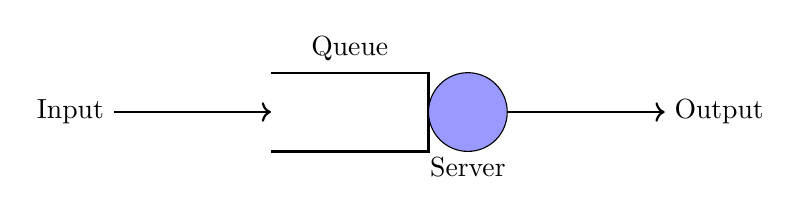
\begin{tikzpicture}
    % Draw the queue block (left-open rectangle)
    \draw[thick] (0, 0.5) -- (2, 0.5) -- (2, -0.5) -- (0, -0.5);
    \node at (1, 0.8) {Queue};

    % Draw the input arrow
    \draw[->, thick] (-2, 0) -- (0, 0);
    \node[left] at (-2, 0) {Input};

    % Draw the server (circle)
    \filldraw[fill=blue!40, draw=black] (2.5, 0) circle (0.5);
    \node at (2.5, -0.7) {Server};

    % Draw the output arrow
    \draw[->, thick] (3, 0) -- (5, 0);
    \node[right] at (5, 0) {Output};
\end{tikzpicture}
    \caption{Block diagram of a simple, 1-D queue with one server and infinite capacity.}
    \label{fig:simpleQblk}
\end{figure}

\subsection{Block diagram}
A queue is frequently depicted in literature as shown in Fig.\ref{fig:simpleQblk}.

\subsection{Terminology}
The Fig.\ref{fig:simpleQblk} has a few terms used in it.  A queue is formed by entities, the nature of which depends on the context provided by the application of the theory. For example, it could be jobs waiting to be executed at a server in a data center, humans waiting at a bank, or airplanes at an airport awaiting takeoff. To address the requirements of the entities, there is an object we call a server. This server might be the processor, the bank manager, or the air traffic controller, respectively, in the aforementioned queues.

Whenever a new entity is added to the queue, we say that an arrival has occurred. When the server addresses an entity, we say that a departure event has occurred. In these notes, we will refer to the entities in the queues as either arrivals or customers.

The state of the queue at any given instant is defined by the number of customers at that moment. This includes those waiting in the queue for their turn at the server, as well as the one currently being served by the server. We will be using a state diagram quite frequently and hope that the reader is comfortable with it. If not, it is recommended that you refer to the relevant chapters in \cite{pishro2014introduction}.

\subsection{Assumptions}
To make our life easy we make a few seemingly trivial yet important assumptions \cite{myReference}:
\begin{enumerate}
    \item If a server is free, an arriving customer directly goes into service. If a server is not free, the customer waits in the queue waiting for its turn at the server. 
    \item When a server becomes free, the next customer is chosen according to a \emph{scheduling policy}.
    \item Customers remain in the ``queueing facility'' once they have been accepted in it and do not become impatient and leave.
\end{enumerate}

\subsection{Kendall Notation}
A queue is characterized by how entities arrive to it, how they depart from it, how many servers are present, and if existant, what is the maximum length of the queue limited to, etc. \emph{Kendall's Notation} provides a condensed way to represent a queue. The general form is given by 
\begin{subequations}
    \begin{align}
        \mA/ \mB/ c/ \mX/ \mY/ \mZ 
    \end{align}
    where, 
    \begin{align*}
        \mA &= \text{Describes arrival statistics.}\\
        \mB &= \text{Describes the departure statistics.} \\
        c &= \text{Number of Servers.}\\
        \mX &= \text{Maximum length of the queue, more commonly known as \emph{system capacity}.}\\
        \mY &= \text{Size of the customer population}. \\
        \mZ &= \text{Queue scheduling discipline.}
    \end{align*}
\end{subequations}
A frequently used statistics is \emph{Markovian}, where the process(es) of arrival and/or departure are Markov. `M' is used to abbreviate a Markovian statistics, `D' to denote Deterministic Timing, `E' for Erlang,`G' for general statistics and `Geom' for Geometric. 

\subsection{Assumptions}

For our purposes of analysis, we make the following assumptions:
\begin{enumerate}
    \item If the server is not serving a customer i.e., it is free, then the arriving (next in line) customer is immediately assigned that server.
    \item Unless mentioned otherwise, if a server is busy, any new arrival joins the queue and waits for its chance.
    \item The time between the departure of a serviced customer and the start of the next customer is zero.
\end{enumerate}
Also, for simplicity, we will be sticking to a first-order analysis, thus, trading modeling accuracy for tractability and thereby insights.

\section{Service Discipline}
One thing we haven't addressed so far, is the order in which the customers in a queue are called for service. 
\dfn{Scheduling Discipline}{
    The rule that decides which customer in the queue will be serviced after a departure is known as the scheduling discipline.

    This rule is also referred to as the scheduling algorithm or scheduling policy in the literature.
}
One obvious rule is First Come First Serve (FCFS), also known as First-In-First-Out (FIFO). However, there are scenarios where different disciplines are implemented. For example, in mobile communication networks, emergency notifications regarding disasters must be prioritized over all other messages. In this case, the system might follow Last-In-First-Out-Pre-Emptive-Resume (LIFOPR). Readers associated with embedded systems or computer architecture may be familiar with the ``memory stack'' which is used to manage interrupts or function calls. In this case, the order in which different routines are serviced depends on the priorities of the interrupts, in addition to the order in which they are triggered (LIFO is the most commonly used discipline).

For our purposes, we will keep it simple and limit ourselves to the FIFO service discipline. Now will look at a few queues with models that provide feasible and tractable mathematical models.

\chapter{M/M/1 Queue}
In this chapter, we will study the simplest kind of queue, the $M/M/1$ or also known as \emph{Markovian} queue. While the queue, once we delve into its details, may not seem entirely realistic, it provides valuable insights due to its mathematical tractability.

\dfn{M/M/1 (or Markovian) Queue}{
    A $M/M/1$ queue, also known as \emph{Markovian} queue is characterized as follows:
    \begin{enumerate}
        \item The arrival process follows a Poisson random process.
        \item There is a single server, with the service times for each customer being independent and exponentially distributed. 
        \item There is no limit on the size of the queue. Additionally, the state of the queue is given by the number of arrivals/customers in the queue at a given moment.
    \end{enumerate}  
}

Its our first queue under study, let's understand this queue slowly, building the model step by step.

\section{Arrivals}
By definition, the arrivals in an $M/M/1$ queue are a Poisson random process. If you are not familiar, its okay, since we will derive the entire framework from basic probability and a little bit of imagination. However, you may refer \cite{pishro2014introduction} for more details.

\subsection{Poisson Random Arrival Process}
Consider an experiment where you are observing a queue and tracking its movement. For simplicity, you divide the time axis into smaller intervals of length $\delta t$, such that at most one arrival can occur within each interval, or there may be no arrival at all. What decides whether there is an arrival or not? You toss a magical coin that is weirdly biased. If the toss results in heads, there is an arrival at the queue; otherwise, there is no arrival. The bias of the coin landing on heads is proportional to the length of the time interval, i.e., 
$$\mathbb{P}(\text{Heads}) = \lambda \times \delta t,$$ 
where $\lambda$ is a constant. Now, if we consider an interval of length $T$, the number of slots (or small $\delta t$ intervals) within that time interval is approximately, 
$$n \approx \frac{T}{\delta t}.$$ 
Therefore, the experiment reduces to $n$ coin flips, each with a bias of $\lambda \delta t$. 

The state of the system is given by the number of customers in the queue, $N(t)$ at some time instant $t$. From the coin analogy, we see that $N(t) \sim \text{Binomial}(n, p=\lambda\delta t)$
\begin{align}
    P_{N(t)}(k) &= \sP(N(t) = k) = \sP(\text{k arrivals in the interval [0, t]}) \\
    &= {n \choose k} (\lambda \delta t)^{k} (1 - \lambda \delta t)^{n-k} 
\end{align} 
Taking limit as $\delta t   \rightarrow 0$ and $\delta t \approx t / n$ (this implies that $n \rightarrow \infty$),
\begin{align}
    \lim_{\delta t \rightarrow 0} P_{N(t)}(k) &= \lim_{\delta t \rightarrow 0} \frac{n!}{k! (n-k)!} \frac{\lambda^{k} t^{k}}{n^k} \left( 1 - \frac{\lambda t}{n} \right)^{n-k} \\
    &= \lim_{n \rightarrow \infty} \frac{n \times (n-1) \times (n-2) \times \dots \times (n-(k-1))}{k!} \frac{\lambda^{k} t^{k}}{n^k} \left( 1 - \frac{\lambda t}{n} \right)^{n-k} \\
    &= \frac{1}{k!} \lim_{n \rightarrow \infty} \left( \frac{n}{n} \times \frac{n-1}{n} \times \frac{n-2}{n} \times \dots \times \frac{n-(k-1)}{n} \right) \lambda^{k} t^{k} \left( 1 - \frac{\lambda t}{n} \right)^{n-k} \\
    &= \frac{1}{k!} \lim_{n \rightarrow \infty} \left( 1 \times \left( 1 - \frac{1}{n} \right) \times \left( 1 - \frac{2}{n} \right) \times \dots \times \left( 1 - \frac{k-1}{n} \right) \right) \lambda^{k} t^{k} \left( 1 - \frac{\lambda t}{n} \right)^{n-k} \\
    &= \frac{\lambda^{k} t^{k}}{k!} \lim_{n \rightarrow \infty} \left( 1 - \frac{\lambda t}{n} \right)^{n-k} \\
    &= \frac{\lambda^{k} t^{k}}{k!} \lim_{n \rightarrow \infty} \left( 1 - \frac{\lambda t}{n} \right)^{n} \\
    &= \frac{\lambda^{k} t^{k}}{k!} e^{-\lambda t}
\end{align}


Thus, we get the result, 
\begin{align}
    P_{N(t)}(k) \sim \text{Poisson}(\lambda t) 
\end{align}

Lets make a few observations.
\begin{subequations}
    \begin{align}
        P_{N(\delta t)}(0) &= e^{-\lambda \delta t} \\
        &= 1 - \lambda \delta t + (\lambda \delta t)^2 - \ldots &&\quad \ldots \text{Taylor series expansion of } e^x.\\
        &\approx 1 - \lambda \delta t &&\quad \ldots \text{Neglecting higher order terms}.\\
        \\
        P_{N(\delta t)}(1) &= \lambda \delta t e^{-\lambda \delta t} \\ 
        &= \lambda \delta t (1 - \lambda \delta t) \\
        &= \lambda \delta t\ &&\quad\ \ldots\text{Ignoring higher order terms.}\\
        \\
        P_{N(t)}(k \geq 1) &\approx 0
    \end{align}    
    \label{eq:ApproxAssumptions}
\end{subequations}
Thus, we see that in the small interval $\delta t$, there is at most one arrival with probability of $\lambda \delta t$. Also there cannot be more than one arrival in the small interval.

\subsection{State of the System - Alternative approach}
I would like to emphasize again that we are still considering only the arrivals and the state of the system is given by the number of customers in the system at a paticular time.

We can derive the distribution alternatively starting from Equations \ref{eq:ApproxAssumptions} as the basic setup or assumptions. 

\begin{figure}
    \centering
    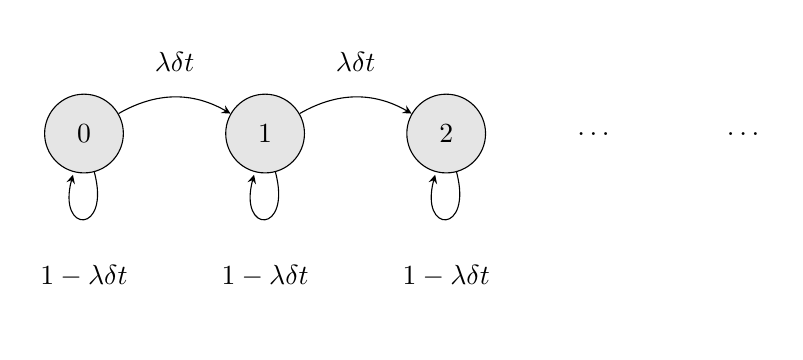
\begin{tikzpicture}[>=stealth, node distance=2.3cm, every node/.style={circle}]
    % Nodes
    \node (0) [draw, fill=gray!20, minimum size=10mm] {0};
    \node (1) [right of=0, draw, fill=gray!20, minimum size=10mm] {1};
    \node (2) [right of=1, draw, fill=gray!20, minimum size=10mm] {2};

    % Infinite continuation
    \node (ellipsis) [right of=2, xshift=1.5cm] {\dots};

    % Connecting nodes with edges and labels as plain text
    \path[->] (0) edge [bend left] node[above] {$\lambda \delta t$} (1)
              (1) edge [bend left] node[above] {$\lambda \delta t$} (2)
              ;

    % Self-loops with labels as plain text
    \path[->] (0) edge [loop below] node[below] {$1 - \lambda \delta t$} (0)
              (1) edge [loop below] node[below] {$1 - \lambda \delta t$} (1)
              (2) edge [loop below] node[below] {$1 - \lambda \delta t$} (2);

    % Ellipses for continuation
    \node at ($(2)!0.5!(ellipsis)$) {\dots};
\end{tikzpicture}

    \caption{State Transition Diagram for only arrivals}
    \label{fig:arrSTD}
\end{figure}

If $\sP(\text{Number of customers in the queue} = k, \text{at time}\ t) = P_{k}(t)$, then in a single $\delta t$ interval we can reach a state by either a single arrival or no arrival. We denote $p_{i,j}$ as the transition probability of going from state $i$ to $j$ in a $\delta t$ interval.
\begin{subequations}
    \begin{align}
        P_n(t+\delta t) &=  P_n(t)p_{n,n} + P_{n-1}(t)p_{n-1, n} \\
        &= P_n(t)(1 - \lambda \delta t) + P_{n-1}(t) (\lambda \delta t) &&\quad\ \ldots\ \text{See Fig.\ref{fig:arrSTD}} \\
        P_0(t + \delta t) &= P_0(t)p_{0, 0} \\
        &= P_0(t)(1 - \lambda \delta t)
    \end{align}
    \label{eq:altDer01}
\end{subequations}
Thus, we arrive at a recursive equation. However, we still need a starting (boundary) condition in order to get a solution. For this, note that to be at state 0, the system must have no arrival starting at state 0 (only arrivals remember?). Reorganizing Equations \ref{eq:altDer01},
\begin{subequations}
    \begin{align}
        \frac{P_n(t+\delta t) - P_n(t)}{\delta t} &= -\lambda P_n(t) + \lambda P_{n-1}(t) \\
        \frac{d P_n(t)}{dt} &= -\lambda P_n(t) + \lambda P_{n-1}(t) &&\quad\ \ldots\ \delta t \rightarrow 0.
    \end{align}
    Case $n = 0$ :
    \begin{align}
        \frac{d P_0(t)}{d t} = -\lambda P_0(t)
    \end{align} 
    Now, those who are comfortable with and accustomed to working with differential equations may solve the above equation by visual inspection. Others may verify the solution by plugging the alleged function into the differential equation and checking that it satisfies the equation. The solution is,
    \begin{align}
        P_0(t) = e^{-\lambda t}
    \end{align} 
    Similarly, 
    Case $n = 1$:
    \begin{align}
        \frac{d P_1(t)}{d t} &= \lambda P_1(t) + \lambda e ^{-\lambda t} \\
        P_1(t) &= \lambda t e^{-\lambda t}
    \end{align}
    Recognizing a pattern, we can generalize the result without explicit proof (provided by induction in \cite{myReference}) as,
    \begin{align}
        P_n(t) = \frac{(\lambda t)^n}{n!} e^{-\lambda t}
    \end{align}
\end{subequations}
Thus, we reach the same result that we derived in the previous section. The difference is that we started from two different, yet equivalent, definitions of the Poisson random process.

\nt{The Poisson random process has \emph{independent increments} and \emph{stationary increments}\cite{pishro2014introduction}. This, means that the number of arrivals in two disjoint time intervals are independent and the associated statistics are time-invariant, i.e., they depend only on the length of the interval.}

Modeling a queue using such statistics has a fair share of advantages. Other than easy mathematical derivations, it is useful that splitting (thinning) and aggregation of Poisson random processes results in other independent Poisson random processes. See the appendix if you are unfamiliar with splitting and merging of Poisson random processes. 

\qs{\cite{RobertazziQ}}{If a telephone exchange is known to receive 100 calls a minute on average, what is the probability, that it gets 0 calls in 5 seconds.\\
\sol 0.00024.}

Now that we have the distribution of the state of the queue, we can find a few statistics that might help us in making decisions. We begin by finding the mean number of customers in the queue, denoted by $\bar{N}$.

\subsection{Mean number of arrivals in an interval $[0, t]$}
\begin{subequations}
    \begin{align}
        \bar{N}(t) &= \ExpVal[N(t)] \\
        &= \sum_{n=0}^{\infty} n P_n(t) \\
        &= \sum_{n=0}^{\infty} n \times \frac{(\lambda t)^n}{n!} e^{-\lambda t} \\
        &= e^{-\lambda t} (\lambda t) \sum_{n=1}^{\infty} \frac{(\lambda t)^{n-1}}{(n-1)!} \\
        &= e^{-\lambda t} (\lambda t) \sum_{n=0}^{\infty} \frac{(\lambda t)^n}{n!} \\
        &=  e^{-\lambda t} (\lambda t) e^{\lambda t} &&\quad\ \ldots\ \text{Taylor Series expansion of }e^x.\\
        \therefore \bar{N}(t) &= \lambda t
    \end{align}
    \label{eq:Meanarr}
\end{subequations}

\nt{
    - The result obtained is intuitively satisfactory, since it states that, on average, the number of customers in a queue is proportional to the time interval of interest.
    Let us now see what this proportionality constant means.
}

\qs{What does the proportionality constant $\lambda$ signify?}{
    \sol{Consider the average number of arrivals per unit time i.e., 
    \begin{subequations}
        \begin{align}
            \bar{N} &= \frac{1}{t} \ExpVal[N(t)] \\
            \bar{N} &= \frac{1}{t} \sum_{k = 0}^{\infty} k P_{N(t)}(k) \\
            &= \frac{1}{t}\lambda t \\
            &= \lambda 
        \end{align}
    \end{subequations}
Hence, $\lambda$ is the rate of arrivals or mean arrivals per unit time.} 
}

\subsection{Variance of Number of arrivals in an interval $
[0, t]$}
Consider,
\begin{subequations}
    \begin{align}
        \ExpVal[N(t)^2] &= \sum_{n=0}^{\infty} n^2 \frac{(\lambda t)^n}{n!}e^{-\lambda t} \\
        &= \sum_{n=1}^{\infty} n^2 \frac{(\lambda t)^n}{n!}e^{-\lambda t} \\
        &= \sum_{n=1}^{\infty} n \frac{(\lambda t)^n}{(n-1)!}e^{-\lambda t} \\
        &= (\lambda t)e^{-\lambda t} \sum_{n=1}^{\infty}n \frac{(\lambda t)^{n-1}}{(n-1)!} \\
        &= (\lambda t)e^{-\lambda t} \sum_{n=0}^{\infty}(n+1) \frac{(\lambda t)^{n}}{(n)!} \\
        &= (\lambda t)e^{-\lambda t} \big[\sum_{n=0}^{\infty}n \frac{(\lambda t)^{n}}{(n)!}+ \sum_{n=0}^{\infty} \frac{(\lambda t)^{n}}{(n)!}\big] \\
        &= \lambda t e^{-\lambda t} [\lambda t e ^{\lambda t} + e^{\lambda t}] \\
        &= \lambda (1 + \lambda t) \\
        &= \lambda t + \lambda^2 t^2 \\
        \therefore var(N) &= \lambda t + \lambda^2 t^2 - (\lambda t)^2 \\
        &= \lambda t.
    \end{align}
    \label{eq:varArrivals}
\end{subequations}

\subsection{Inter-arrival times}

\dfn{Interarrival Time}{
    The time elasped between two consecutive arrival events is called the Inter-arrival time between those two events. Note that this is a stochastic quantity in our model.
}
Let $T$ denote the interarrival time. Thus we begin by finding the cumulative distribution function (CDF) of $T$, 
\begin{subequations}
    \begin{align}
        F_T(t) = \sP(T \leq t) &= \sP(\text{Interarrival time is less than or equal to } t) \\
        &= 1 - \sP(\text{Interarrival time is more than } t) \\
        &= 1 - \sP(\text{No arrival in time interval of length } t) \\
        &= 1 - P_0(t) \\
        &= 1 - e^{-\lambda t}  
    \end{align}
    We recognize this CDF as that of an \emph{exponentially} distributed random variable. If you don't, we can get the PDF (which hopefully you will be more familiar with) by differentiating as, 
    \begin{align}
        f_T(t) = \frac{d F_T(t)}{dt} = \lambda e^{-\lambda t}
    \end{align}
    Thus, the interarrival time $T$ is distributed as 
    \begin{align}
        T \sim \text{Exponential}(\lambda).
    \end{align}
    \label{eq:intertime}
\end{subequations}
Now's a good time to make some observations.
\nt{
    \begin{enumerate}
        \item The inter-arrival times are exponentially distributed, meaning that the system is memoryless (see \cite{pishro2014introduction}). Intuitively, the current state of the system does not depend on the past. More concretely, say $\lambda = 10$ min, and we have had no arrival for 6 minutes since we started observing. Then, the time after which we expect an arrival is still 10 minutes from now, not 4 minutes! This means it is as if we are starting a new observation window. I recommend that you go through the proof of the memorylessness property of the exponential distribution in \cite{pishro2014introduction}, as it is quite simple.
        \item Due to this, the state of the system at any given instant is completely determined by the number of customers in the queue at that instant; there is no conditional dependence on the past.
        \item A discrete distribution with the memoryless property is the Geometric distribution.
    \end{enumerate}
    
}

\section{Service}
We have ignored the server for a long time. Let's include it in our model now. In our $M/M/1$ model, we make the assumption that the service times for every customer are independent and identically distributed exponential random variables with rate $\mu$.

Thus, we make the following assumptions in addition to our previous ones.
\begin{subequations}
    \begin{align}
        \sP(\text{exactly 1 service in} [t, t+\delta t]) &= \mu \delta t \\
        \sP(\text{no service in} [t, t+\delta t]) &= 1 - \mu \delta t  \\
        \sP(\text{more than 1 service in} [t, t+\delta t]) &= 0.  
    \end{align}    
    \label{eq:assumDep}
\end{subequations}
Now the state of the system will be given by the number of customers in the queue as well as the one in service. 

The process resulting from such a system is called a \emph{birth-death} process in the literature\cite{RobertazziQ, myReference}. The state transition diagram can be now updated to include the departures as well. See Fig.\ref{fig:mm1_std}. 
\begin{figure}
    \centering
    \begin{tikzpicture}[>=stealth, node distance=2.3cm,every node/.style={circle}]
    % Nodes
    \node (0) [draw, fill=gray!20, minimum size=10mm] {0};
    \node (1) [right of=0, draw, fill=gray!20, minimum size=10mm] {1};
    \node (2) [right of=1, draw, fill=gray!20, minimum size=10mm] {2};
    \node (3) [right of=2] {\dots};

    % Connecting nodes with edges and labels as plain text
    \path[->] (0) edge [bend left] node[above] {$\lambda$} (1) 
              (1) edge [bend left] node[above] {$\lambda $} (2)
              (2) edge [bend left] node[above] {$\lambda $} (3)
              ;

    \path[->] (1) edge [bend left] node[below] {$\mu$} (0)
    (2) edge [bend left] node[below] {$\mu$} (1)
    (3) edge [bend left] node[below] {$\mu$} (2)
    ;
    % Ellipses for continuation
    \node at ($(2)!0.5!(ellipsis)$) {\dots};
\end{tikzpicture}

    \caption{State Diagram for an $M/M/1$ system.}
    \label{fig:mm1_std}
\end{figure}

\subsection{State of the System}
Using the previous notation and the differential equation approach, we now include the possibility of a departure as well. Remember, we can only jump between adjacent states in a single $\delta t$ interval. Also, when we are in state 0, we can either stay in state 0 or depart to state 1.
Thus, we get the equations,
\begin{subequations}
    \begin{align}
        P_n(t + \delta t) &= P_n(t) p_{n, n} + P_{n-1}(t)p_{n-1, n} + P_{n+1}(t) p_{n+1, n} \\
        P_0(t + \delta t) &= P_0(t)p_{0, 0} + P_1(t)p_{1, 0}
    \end{align}
    Now, 
    \begin{align}
        p_{n, n} &= \sP(\text{(No arrival and no departure) or (One arrival and One departure)}) \\ 
        &= (1 - \lambda \delta t)(1 - \mu \delta t) + (\lambda \delta t)(\mu \delta t) \\
        &\approx 1 - \lambda \delta t - \mu \delta t \\
        p_{n-1, n} &= \sP(\text{One arrival and no departure}) \\
        &= (\lambda \delta t)(1 - \mu \delta t) \\
        &\approx \lambda \delta t \\
        p_{n+1, n} &= \sP(\text{One departure and no arrival})\\
        &= (\mu \delta t)(1 - \lambda \delta t) \\
        & \approx \mu \delta t.  
    \end{align}  
    \label{eq:stateMM1}
\end{subequations}
\nt{Higher order terms have been neglected for a first order analysis. Also, we cannot have a departure in state 0.}
Similar to the previous derivations, we obtain
 the following differential equations:
\begin{subequations}
    \begin{align}
        \frac{d P_n(t)}{d t} &= -(\lambda + \mu) P_n(t) + \lambda P_{n-1}(t) + \mu P_{n+1}(t) \\
        \frac{d P_0(t)}{d t} &= -\lambda P_0(t) + \mu P_{1}(t) 
    \end{align}
\end{subequations}
Solving these equations can be arduous especially for the transient phase of the system i.e., when the state probabilities have not settled or become \emph{stationary}. For a first-cut analysis we are satisfied with the stationary distribution or the state probabilities when the system has reached equilibrium.
\qs{When does a Markov chain achieve equilibrium?}{
    \sol{
        It is apparent from the state diagram, Fig.\ref{fig:mm1_std}, that we are dealing with a discrete time Markov chain. A Markov chain is said to be in equilibrium or stationary when the state distribution is no longer time-variant. It is this distribution that we are most interested about. Moving forward, we will only concentrate on finding the stationary distributions.  
    }
}
The formation of differential equations though easy was time consuming. Now we define a new quantity called \emph{Probability Flux} that will help us form recursive equations of the stationary distributions which we can easily solve. 

\dfn{Probability Flux \cite{RobertazziQ}}{
    Probability Flux is defined as the product of the probability of being in the state at which a transition originates and the transition rate to which the state travels next.

    It can be physically understood as the mean number of transitions that occur per unit time. For example, if $\lambda = 10\ \text{sec}^{-1}$ and probability of being in originating state is $0.5$, then on an average the systems makes that transition five times every second.   
}

Probability flux can be understood better if we make an analogy. However, beware that the following analogy is only a loose one and does not extrapolate to other results. We can relate a node in the state transition diagram to a node in an electrical circuit. Just as Kirchhoff's Current Law states that the current into a node must equal the current out of it, similarly, the flow of transitions into a node of a state transition diagram must equal the flow out of it in equilibrium. The resultant equations that one gets are collectively known as \emph{Global Balance Equations}.

For those not yet convinced, lets just go by the definition of Probability flux. Take a node say node 1 in Fig.\ref{fig:mm1_std}. If we add the probability fluxes together with the signs representing the direction, we get,
\begin{align}
    \Phi_P(\text{node}\ 1) &= \text{Flow out of node } 1 + \text{Flow into node } 1\\
    &= -(\lambda + \mu) p_1 + \lambda p_0 + \mu p_2
\end{align}
If you observe carefully, this is the right-hand side of Eq. (2.20a) for $n = 1$. So, if we are at equilibrium, we expect that the state probabilities be time-invariant, i.e., $\frac{dp_n(t)}{dt} = 0$. Thus, $\Phi_P(\text{node} 1) = 0$, i.e., the total flux into a node equals the total flux out of a node.
We can use these to form recursive equations for the state probabilities at equilibrium and obtain the stationary distribution.

In conclusion, when the system is in equilibrium, the probability flux into a state equals the probability flux out of the state. This is called flow balancing and leads to what are known as the balancing equations.

To further simplify this process, we can form the \text{local balance equation}s which essentially say that the flow toward the right, across a boundary separating two states of a system, equals the flow towards the left\footnote{This process of forming the local balance equations is easy only when the states are 1-D. But when the states are drawn in higher dimensions, it is claimed in \cite{myReference} that a cluster-based approach would be easier. These structures being beyond the scope of these notes have not been verified or even looked into by us.} 

Going back to our queue model, we get the following local balance equations,
\begin{subequations}
    \begin{align}
        \lambda p_0 &= \mu p_1 &&\quad \implies p_1 = \frac{\lambda}{\mu} p_0 \\ 
        \lambda p_1 &= \mu p_2 &&\quad \implies p_2 = \frac{\lambda}{\mu} p_1 \\
        \vdots \\
        \lambda p_{n-1} &= \mu p_n &&\quad \implies p_n = \frac{\lambda}{\mu} p_{n-1} \\
        \vdots \\
    \end{align}
    Thus, we get the general equation\footnote{\cite{myReference} provides an arguably better proof by principle of mathematical induction in our opinion which you may refer.},
    \begin{align}
        p_n = \left(\frac{\lambda}{\mu}\right)^n p_0
    \end{align}
    \label{eq:lclBal}
\end{subequations}
Since the system must be in at least one of the possible states, the axioms of probability give us another equation:
\begin{align}
    \sum_{i=0}^{\text{num}_{\text{states}}} p_i = 1.
\end{align}
Defining $\rho = \frac{\lambda}{\mu}$ for our $M/M/1$ system with an infinite number of states, we get:
\begin{align}
    p_0 + \rho p_0 + \rho^2 p_0 + \ldots &= 1 \\
    \therefore p_0 &= \frac{1}{\sum_{i=0}^{\infty} \rho^i}
\end{align}

Consider the case when $0 \leq \rho < 1$:
\begin{align}
    p_0 &= \frac{1}{\frac{1}{1 - \rho}} \\
    &= 1 - \rho.
\end{align}

\nt{Since $p_0$ is the probability that the queue is empty or unutilized, we call $\rho$ utilization. When $\lambda$ is close to 0, we say we have a very light load or zero load. Alternatively, if $\lambda \rightarrow \mu$, we say we have a heavy load.}

\qs{Is it possible that $\rho > 1$?}{
    \sol{
        No (atleast for reaching equilibrium). From the above derivation we see that the length of the queue will balloon up and blow up to be infinite in size. Hence, the system will not reach equilibrium, invalidating our above assumptions.
    }
}

\dfn{Utilization}{
    In a single server system, Utilization is defined as the fraction of time the server is busy.

    In case of multiple servers, we Utilization as the average fraction of available servers that are busy.   
}

\qs{What is utilization for $M/M/1$ queue? Is it always the same?}{
    \sol{
        Consider a time interval of length $T$. Then the mean arrivals in this time interval will be $\lambda T$. The server serves at an average rate of $\mu$ per unit time. Thus, the amount of time the server will be busy is given by $\lambda T / \mu$.
        Normalizing to find the fraction of time the server is busy, 
        Utilization $ = \frac{1}{T} (\lambda T / \mu) = \lambda / \mu$ which is why $\rho$ is also called utilization.

        In some cases, where customers are denied access to the queue due to a finite buffer size, the utilization is not exactly $\rho$, but slightly less than it, as there are fewer than $\lambda$ mean arrivals due to excess customers being dropped.
    }
}

\subsection{Average number of customers in $M/M/1$ queue}

We will now use the updated distribution (for steady state) that includes the service time distribution as well.
\begin{subequations}
    \begin{align}
        \bar{N} = \mathbb{E}[N] &= \sum_{n=0}^{\infty} n p_n \\
        &= \sum_{n=0}^{\infty} n \rho^n p_0 \\
        &= (1 - \rho) \sum_{n=0}^{\infty} n \rho^n \\
        &= \rho (1 - \rho) \sum_{n=0}^{\infty} n \rho^{n-1} \\
        &= \rho (1 - \rho) \sum_{n=0}^{\infty} \frac{d \rho^n}{d \rho} \\
        &= \rho (1 - \rho) \frac{d}{d \rho} \left( \sum_{n=0}^{\infty}  \rho^n \right) \\
        &= \rho(1 - \rho) \frac{d}{d \rho} \left( \frac{1}{1 - \rho} \right) \\
        &= \frac{\rho}{1 - \rho}
    \end{align}
    \label{eq:avgMM1}
\end{subequations}

\subsection{Variance of number of customers in $M/M/1$ queue}
Consider,
\begin{subequations}
    \begin{align}
        \ExpVal[N^2] &= \sum_{n=0}^{\infty} n^2 (1 - \rho)(\rho^n) \\
        &= (1 - \rho) \big[\sum_{n=0}^{\infty}n(n+1-1)\rho^n \big] \\
        &= (1 - \rho) \big[\sum_{n=0}^{\infty} n(n+1)\rho^n - \sum_{n=0}^{\infty}n\rho^n\big] \\
        &= (1 - \rho) \big[\rho^2 \sum_{n=0}^{\infty} n(n+1)\rho^{n-1} - \rho\sum_{n=0}^{\infty}n\rho^{n-1}\big] \\
        &= (1 - \rho) \big[\rho^2 \sum_{n=0}^{\infty} \frac{d^2\rho^{n+1}}{d\rho^2} - \rho\sum_{n=0}^{\infty}\frac{d\rho^{n}}{d \rho}\big] \\
        &= (1 - \rho) \big[\rho^2 \frac{d^2 \big(\sum_{n=0}^{\infty} \rho^n \big)}{d\rho^2} - \rho \frac{d \big(\sum_{n=0}^{\infty} \rho^n \big)}{d\rho}\big]
    \end{align}
    Using the formula for sum of Geometric Progression (for common ratio $< 1$),
    \begin{align}
        &= (1 - \rho) \big[ \rho^2 \frac{2}{(1-\rho)^3} + \frac{\rho}{(1 - \rho)^ 2}\big] \\
        &= \frac{\rho(1 + \rho)}{(1 - \rho)^ 2} \\
        \therefore \text{var}(N) &= \frac{\rho(1 + \rho)}{(1 - \rho)^ 2} - \frac{\rho^2}{(1 - \rho)^2} \\
        &= \frac{\rho}{(1 - \rho)^2}.
    \end{align} 
    \label{fig:varMM1}
\end{subequations}

\begin{figure}
    % First subfigure: Branching Diagram
    \begin{subfigure}[b]{0.55\textwidth}
        \centering
        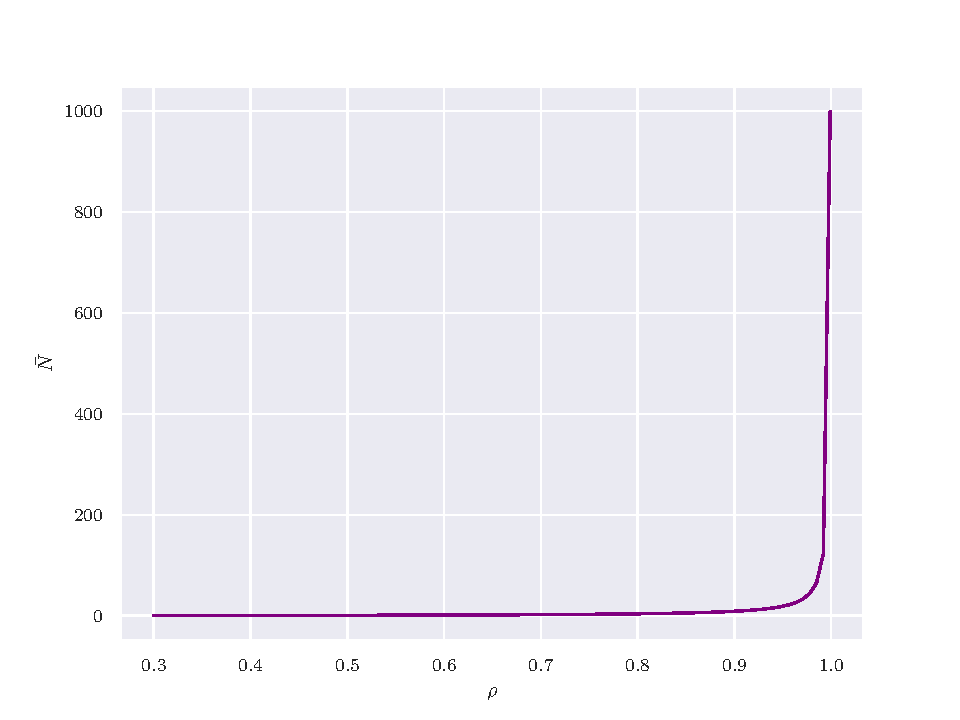
\includegraphics[width=\textwidth]{plots/avg_mm1.pdf}
        \caption{Average number of customers in an $M/M/1$ queue.}
        \label{fig:avgMM1_plot}
    \end{subfigure}
    \hfill
    % Second subfigure: Merging Diagram
    \begin{subfigure}[b]{0.55\textwidth}
        \centering
        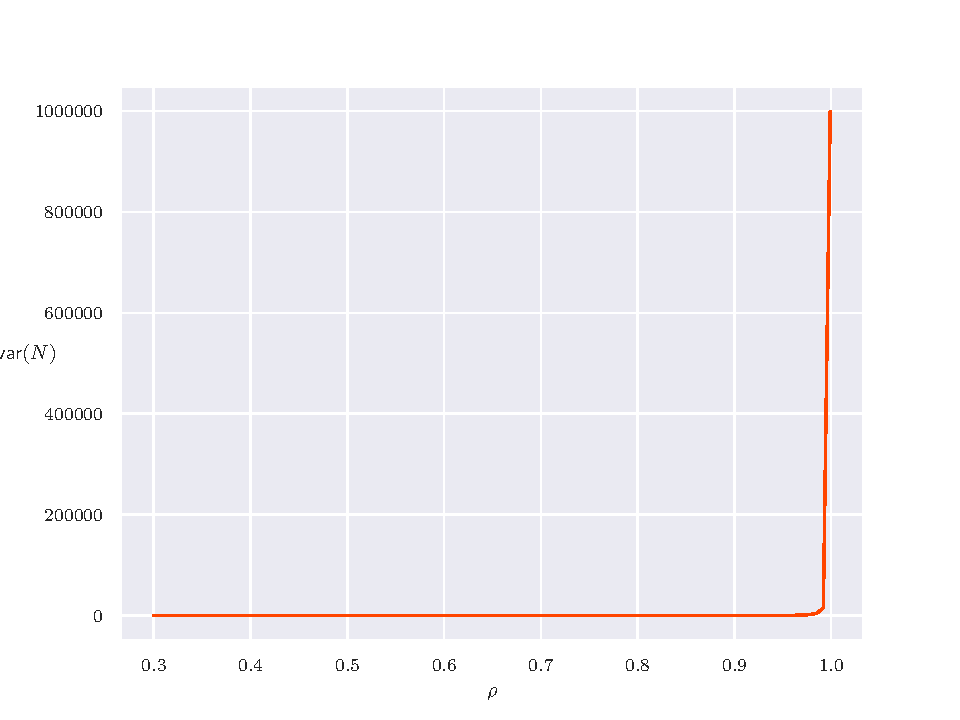
\includegraphics[width=\textwidth]{plots/var_mm1.pdf}
        \caption{Variance of number of customers in an $M/M/1$ queue.}
        \label{fig:varMM1_plot}
    \end{subfigure}
    \label{fig:mm1_stats}
\end{figure}

Please see Figs.\ref{fig:avgMM1_plot} and \ref{fig:varMM1_plot}. Note how the statistics blow up as the Utilization factor approaches 1. Due to the high variance as $\rho \rightarrow 1$, the randomness in the system increases i.e., the unpredictability in the queue is very high. How do you think this might affect analysis of such a queue?

\qs{Where might we use these statistics?}{
    
    \sol{
        As I promised, we will take an approach that will make things clear intuitively. What better way than using a real-life example?

        In a call center, a clever worker who is a queueing theory aficionado could estimate the time between the calls he receives. This would allow him to plan his next coffee break and decide how much time he can spend conversing with a colleague.
        
        More seriously, these statistics are important when it comes to scheduling other regular, low-priority tasks in microprocessor- or microcontroller-based systems. They can be used to plan resources as well. A hospital might decided whether or not a doctor needs an associate. A internet service provider might decide whether or not his infrastucture needs an upgrade.         
        }
}

\section{Little's Law}
Now that we have come so far, lets try to relate the number in the queue with the time dimension.
\thm{Little's Law}{The mean number of customers in the queue, $\bar{N}$ is related to the rate of arrivals, $\lambda$, and the mean service time, $\bar{T}$ as 
\[
\bar{N} = \lambda \bar{T}.
\]
}  
\pf{Proof}{
    Consider a time interval of $[0, T]$.
    \begin{subequations}
        \begin{align}
            &\sP(\text{n customers in the queue after one departure})  \\ 
            &= \sP(\text{n customers arrive during the time spent in the queue by the depart customer.}) \\
            &= \int_{0}^{\infty}\sP(\text{n arrivals in during the interval } [0, T]\ |\ T=t) f_T(t) dt \\
            &= \int_{0}^{\infty}\sP(\text{n arrivals in during the interval } [0, t]) f_T(t) dt  \\
            &= \int_{0}^{\infty} \frac{(\lambda t)^n}{n!} e^{-\lambda t} f_T(t) dt 
        \end{align}
        Now, using formula for expectation of a discrete random variable,
        \begin{align}
            \bar{N} &= \ExpVal[N] \\
            &= \sum_{n=0}^{\infty} nP_n(t) \\
            &= \sum_{n=0}^{\infty} n \int_{0}^{\infty} \frac{(\lambda t)^n}{n!} e^{-\lambda} f_T(t) dt \\
            &= \int_{0}^{\infty} \sum_{n=1}^{\infty} n \frac{(\lambda t)^n}{n!} e^{-\lambda t} f_T(t) dt \\
            &= \int_{0}^{\infty} \sum_{n=1}^{\infty} \lambda t \frac{(\lambda t)^{n-1}}{(n-1)!} e^{-\lambda t} f_T(t) dt \\
            &= \int_{0}^{\infty} \lambda t e^{-\lambda t} f_T(t) \sum_{n=0}^{\infty} \frac{(\lambda t)^n}{n!} dt \\
            &= \int_{0}^{\infty} \lambda t e^{-\lambda t} e^{\lambda t} f_T(t) dt &&\quad\ \ldots\ \text{Taylor series expansion of } e^x. \\ 
            &= \lambda \int_{0}^{\infty} t f_T(t) dt \\
            &= \lambda \ExpVal[T] \\
            &= \lambda \bar{T}.
        \end{align} 
        \label{eq:littleLaw}
    \end{subequations}
}
\nt{This result can be interpreted in simple way. The average waiting, $\bar{T}$, is the amount of time a customer is expected to wait once it arrives at the queue and until it leaves after being serviced. Moreover, $\lambda$ is the mean number of arrivals per unit time. Thus, in the time that a customer is in a queue, is likely to see $\lambda \bar{T}$ customers on an average.}

With this result, we will conclude our study on $M/M/1$ queue. We end with a summary

\section{Summary}
\begin{center}    
    \begin{tabular}{|c|c|}
        \hline
        Random Variable & Distribution \\
        \hline
        \hline
        Number of arrivals in interval (0, t] & $\text{Poisson}(\lambda t)$ \\
        \hline
        Inter-arrival times & $\text{Exponential}(\lambda)$ \\
        \hline 
        Number of departures in the interval (0, t] & $\text{Poisson}(\mu t)$ \\
        \hline
        Inter-departure times & $\text{Exponential}(\mu)$ \\
        \hline
    \end{tabular}
\end{center}
At equilibrium, $\lambda < \mu$, 
\begin{center}
    \begin{tabular}{|c|c|}
        \hline 
        State Probabilities & $p_0 = 1 - \rho$ \\
        & $p_n = \rho^n p_0$ \\
        \hline
        Average number of customers in the queue & $\rho / (1 - \rho)$ \\
        \hline
        Variance of number of customers in the queue & $\rho / (1 - \rho)^2$ \\
        \hline
    \end{tabular}
\end{center}

\chapter{Other Queues}

\section{Limitations of $M/M/1$ model}
While the previous queueing model was simple enough that we could derive the nice results we obtained, it isn't quite realistic. Recall the assumptions we made before embarking on the derivations. One of them was that the coin tosses, which decide whether there is an arrival or not, are independent and thus uncorrelated. However, how realistic is this assumption?

Consider the case of a call center. In my experience, at least, I have hardly ever received any resolution on my first call. What I mean is that once you make a call to a place, it is quite likely that you will call again. This means that the calls are not completely uncorrelated. However, this assumption is acceptable for a first-order analysis.

The next assumption we made was that the queue could, in theory, grow without bound. This is quite unrealistic, simply due to the limited availability of resources and (the doctor's waiting room can't possibly be big enough to have place for infinite patients), not to mention, the patience one would need to endure an infinite human queue. Hence, for the next part of our analysis, we consider a model with finite buffer length.

After this analysis, we ask: why limit our system to a single-server queue? After all, efficiency lies in parallelism. Nowadays, almost all the microprocessors are equipped with multiple cores, essentially multiple compute units. Thus, we consider the cases of $m$ servers and a special case where $m = \infty$.

The analysis in the following sections will be similar to the previous ones and will heavily borrow from those sections. We request that you are comfortable with, and up to speed on, the concepts covered so far.

\section{$M/M/1/N$ - Finite Buffer Queue}

In this model, the queue size is limited to $N$. If there are $N$ customers in the queue, including one in the server, then any new arrivals are turned away or dropped. To maintain the independence of arrivals, we further assume that the dropped customers do not return.

Due to the finite states, we obtain a new state transition diagram, as shown in Fig.~\ref{fig:mm1N_std}.

\begin{figure}
    \centering
    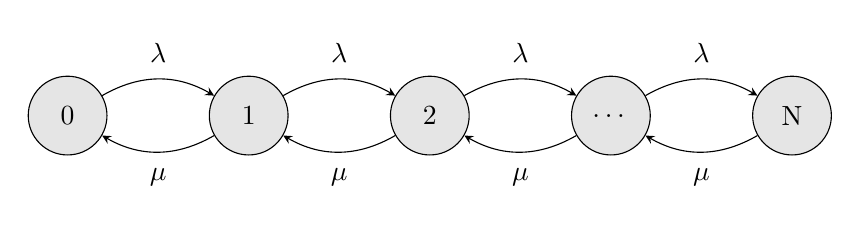
\begin{tikzpicture}[>=stealth, node distance=2.3cm,every node/.style={circle}]
    % Nodes without circles
    \node (0) [draw, fill=gray!20, minimum size=10mm] {0};
    \node (1) [right of=0, draw, fill=gray!20, minimum size=10mm] {1};
    \node (2) [right of=1, draw, fill=gray!20, minimum size=10mm] {2};
    \node (3) [right of=2, draw, fill=gray!20, minimum size=10mm] {$\dots$};
    \node (N) [right of=3, draw, fill=gray!20, minimum size=10mm] {N};

    % Edges with transition rates
    \draw[->, bend left] (0) to node[above] {$\lambda$} (1);
    \draw[->, bend left] (1) to node[above] {$\lambda$} (2);
    \draw[->, bend left] (2) to node[above] {$\lambda$} (3);
    \draw[->, bend left] (3) to node[above] {$\lambda$} (N);

    \draw[->, bend left] (1) to node[below] {$\mu$} (0);
    \draw[->, bend left] (2) to node[below] {$\mu$} (1);
    \draw[->, bend left] (3) to node[below] {$\mu$} (2);
    \draw[->, bend left] (N) to node[below] {$\mu$} (3);

\end{tikzpicture}
    \caption{State transition diagram for $M/M/1/N$ queue.}
    \label{fig:mm1N_std}
\end{figure}

Recollecting the local balance equations, we have under equilibrium,
\begin{subequations}
    \begin{align}
        p_n &= (\frac{\lambda}{\mu})^n p_0 =\rho^n p_0. 
    \end{align}
    Unlike previous model however, $0 \leq n \leq N, (N < \infty)$.
    Thus, to satisfy the axioms of probability, we must have,
    \begin{align}
        p_0 + p_1 + \dots + p_N &= 1 \\
        \implies p_0 + \rho p_0 + \rho^2 p_0 + \dots + \rho^N p_0 &= 1 \\
        p_0 (1 + \rho + \rho^2 + \dots + \rho ^N) &= 1 \\
        p_0 (\frac{1 - \rho ^ {N +1}}{1 - \rho}) &= 1 \\
        \therefore p_0 &= \frac{1 - \rho}{1 - \rho ^ {N + 1}} 
    \end{align} 
    Substituting in {3.1a},
    \begin{align}
        p_n = \big(\frac{1 - \rho}{1 - \rho ^ {N + 1}}\big) \rho ^ n\ \quad\ \ldots\ 0\leq n \leq N.
    \end{align}
    \label{eq:mm1n_eq}
\end{subequations}

\dfn{Blocking Probability}{
    The blocking probability is the probability that the queue buffer is full, i.e., $P_N$. Using the derived equations, Blocking Probability is $\frac{(1-\rho)}{(1 - \rho^{N+1})} \rho^N$ when the system is in equilibrium.
}
\nt{
    Using the blocking probability, we can find the mean number of customers turned away per unit time as $\lambda P_N$.
}

\qs{What is $p_n$ when $\lambda / \mu = 1$?}{
    \sol{
        When $\lambda / \mu = 1$, $p_n$ takes the form $0/0$. We apply L'Hospital's rule:
        \begin{align}
            \lim_{\rho \rightarrow 1} p_n &= \lim_{\rho \rightarrow 1} \frac{1 - \rho}{1 - \rho^{N + 1}}\rho^n \\
            &= \lim_{\rho \rightarrow 1} \frac{1 - \rho}{1 - \rho^{N + 1}} \\
            &= \lim_{\rho \rightarrow 1} \frac{-1}{-(N + 1)\rho^N} \\
            &= \frac{1}{N + 1}.
        \end{align}
    }
}

\nt{
    In this case, since the buffer size is limited, we can have $\lambda > \mu$ as the excess arrivals will simply be turned down or blocked and the queue size will not grow without bounds. 
}

\begin{figure}
    % First subfigure: Branching Diagram
    \begin{subfigure}[b]{0.55\textwidth}
        \centering
        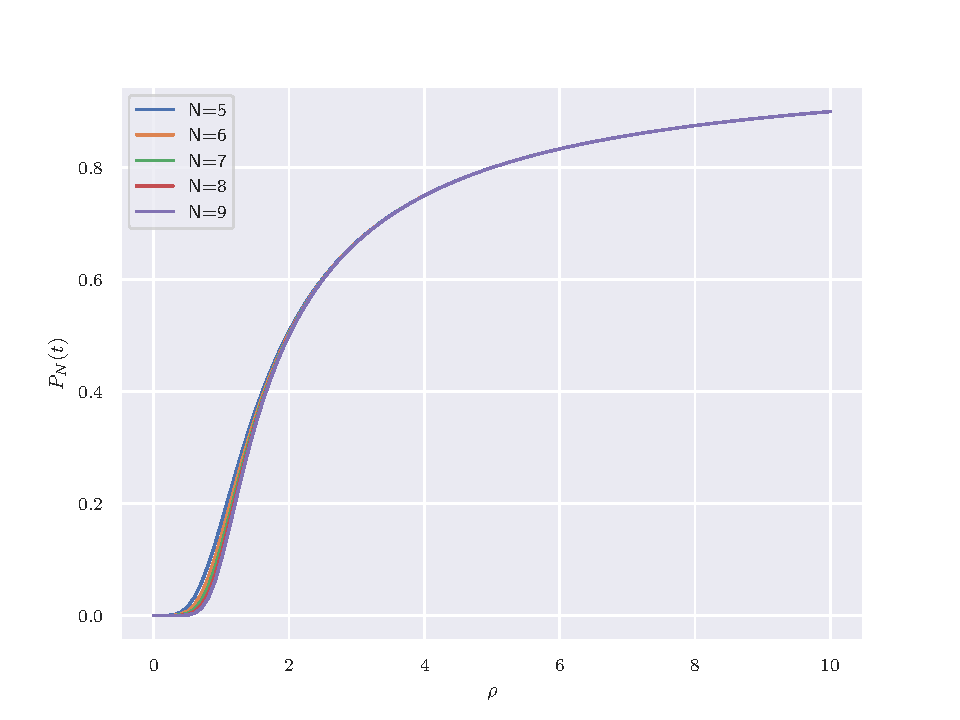
\includegraphics[width=\textwidth]{plots/blockProb_Nfix.pdf}
        \caption{Blocking probability as a function of $\rho$ ($N$ fixed).}
        \label{fig:blkprob_N}
    \end{subfigure}
    \hfill
    % Second subfigure: Merging Diagram
    \begin{subfigure}[b]{0.55\textwidth}
        \centering
        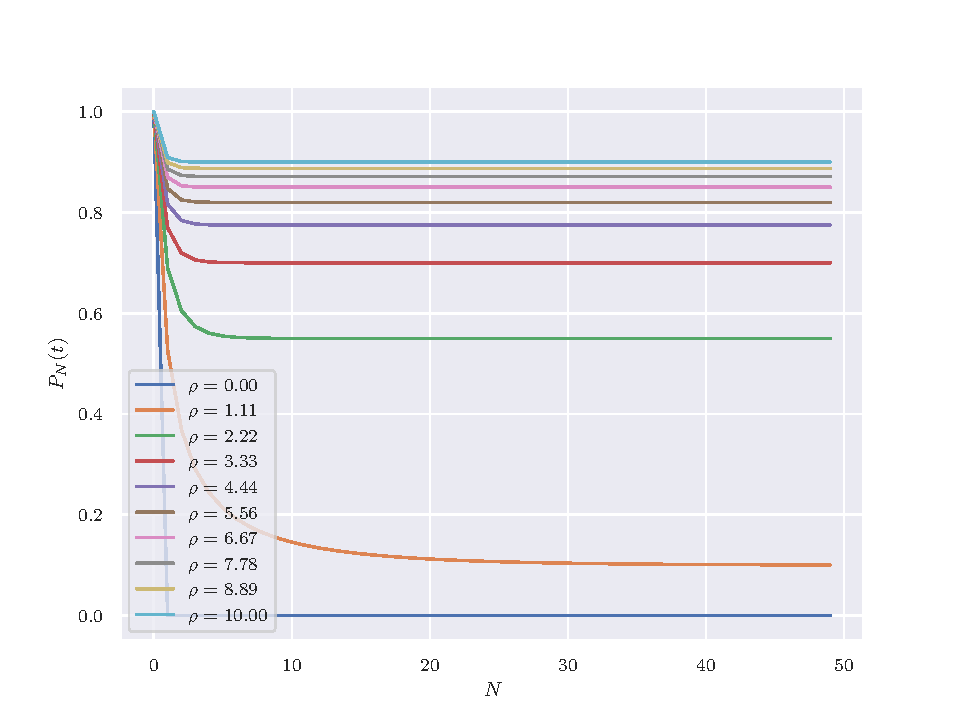
\includegraphics[width=\textwidth]{plots/blockProb_rhofix.pdf}
        \caption{Blocking probability as a function of $N$ ($\rho$ fixed).}
        \label{fig:blkprob_rho}
    \end{subfigure}
    \label{fig:blk_prob}
\end{figure}

We plot the blocking probabilities in Fig.\ref{fig:blkprob_N} and \ref{fig:blkprob_rho}. It concurs with our intuition that the blocking probability increases with increasing utilization ($\rho$) and decreases with increasing buffer length, $N$.

\section{$M/M/\infty$ - Infinite servers}

Now, we move on to the case of multiple server models. However, to begin with, it is easier to consider the infinite server case, as we will soon see. The setup we now have is such that every arriving customer is assigned a personal server with rate $\mu$. Since we have an infinite number of servers, we don't mind if the queue size increases without bound.

\nt{
    If the system has $n$ customers at a time instant, as a whole the system has an aggregate output rate of $n\mu$. 
}
\begin{figure}[ht]   
    \begin{subfigure}[b]{0.55\textwidth}
        \centering
        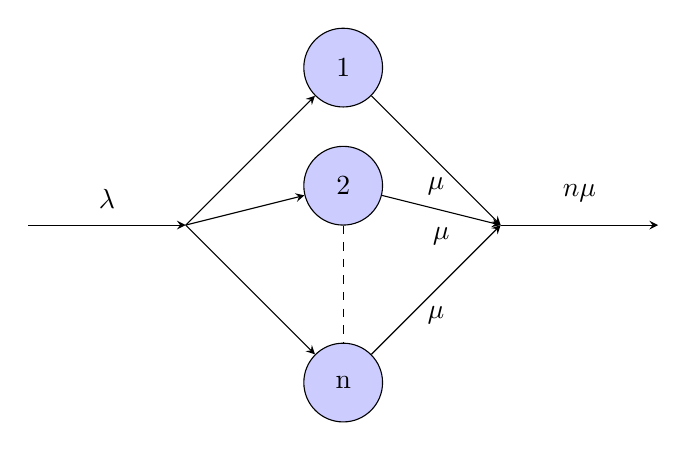
\begin{tikzpicture}[>=stealth, node distance=1.5cm, every node/.style={circle}]
    % Nodes
    \node (1) [{draw, fill=blue!20, minimum size=10mm, inner sep=0pt}]{1};
    \node (2) [{below of=1, draw, fill=blue!20, minimum size=10mm, inner sep=0pt}] {2};
    \node (n) [{below of=2, yshift=-1cm, draw, fill=blue!20, minimum size=10mm, inner sep=0pt}] {n};

    % Arrows for transitions
    \draw[->] (-2, -2) -- (1); 
    \draw[->] (-2, -2) -- (2); 
    \draw[->] (-2, -2) -- (n); 
    \draw[->] (1) -- (2, -2) node[midway, below] {$\mu$};
    \draw[->] (2) -- (2, -2) node[midway, below] {$\mu$};
    \draw[->] (n) -- (2, -2) node[midway, below] {$\mu$}; 

    % Connecting lines between nodes
    \draw[dashed] (2) -- (n);

    % Lambda arrow entering the chain
    \draw[->] (-4, -2) -- (-2, -2) node[midway, above] {$\lambda$};
    \draw[->] (2, -2) -- (4, -2) node[midway, above] {$n \mu$};
    
\end{tikzpicture}
        \caption{Flow diagram of an $M/M/\infty$ queue.}
        \label{fig:blk_mminfinite}
    \end{subfigure}
    \hfill
    \begin{subfigure}[b]{0.55\textwidth}
        \centering
        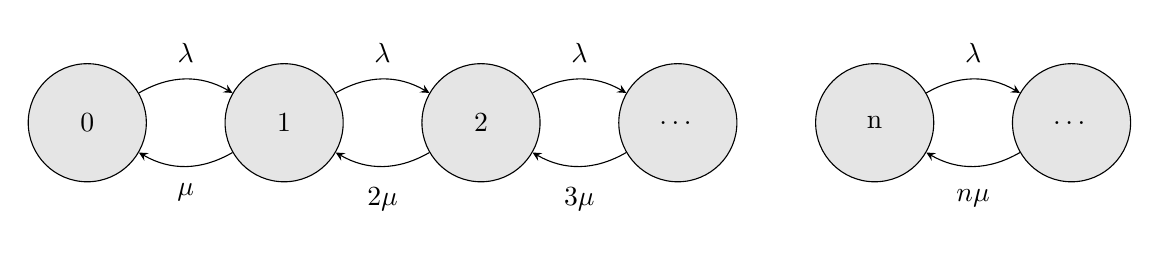
\begin{tikzpicture}[>=stealth, node distance=2.5cm, every node/.style={circle}]
    % Nodes
    \node (0) [{draw, fill=gray!20, minimum size=15mm, inner sep=0pt}] {0};
    \node (1) [{right of=0, draw, fill=gray!20, minimum size=15mm, inner sep=0pt}] {1};
    \node (2) [{right of=1, draw, fill=gray!20, minimum size=15mm, inner sep=0pt}] {2};
    \node (3) [{right of=2, draw, fill=gray!20, minimum size=15mm, inner sep=0pt}] {$\dots$};
    \node (n) [{right of=3, draw, fill=gray!20, minimum size=15mm, inner sep=0pt}] {n};
    \node (dots) [{right of=n, draw, fill=gray!20, minimum size=15mm, inner sep=0pt}] {$\dots$};

    % Transition arrows for arrivals
    \draw[->] (0) to[bend left] node[above] {$\lambda$} (1);
    \draw[->] (1) to[bend left] node[above] {$\lambda$} (2);
    \draw[->] (2) to[bend left] node[above] {$\lambda$} (3);
    \draw[->] (n) to[bend left] node[above] {$\lambda$} (dots);

    % Transition arrows for departures
    \draw[->] (1) to[bend left] node[below] {$\mu$} (0);
    \draw[->] (2) to[bend left] node[below] {$2\mu$} (1);
    \draw[->] (3) to[bend left] node[below] {$3\mu$} (2);
    \draw[->] (dots) to[bend left] node[below] {$n\mu$} (n);
\end{tikzpicture}

        \caption{State transition diagram of an $M/M/\infty$ queue.}
        \label{fig:std_mminfinite}
    \end{subfigure}
    \label{fig:mminfinite_dig}
\end{figure}
Using this setup, and referring to the state transition diagram shown in Fig.~\ref{fig:std_mminfinite}, we get the following local balance equations:
\begin{subequations}
    \begin{align}
        \lambda p_0 &= \mu p_1  &&\implies p_1 = \frac{\lambda}{\mu} p_0 \\
        \lambda p_1 &= 2\mu p_2  &&\implies p_2 = \frac{\lambda}{2\mu} p_1 \\
        \lambda p_2 &= 3\mu p_3  &&\implies p_3 = \frac{\lambda}{3\mu} p_2 \\
    \end{align}
    Generalizing, we get:
    \begin{align}
        p_n &= \frac{\lambda}{n \mu} p_{n-1} \\
        &= \frac{\lambda}{n \mu} \cdot \frac{\lambda}{(n - 1) \mu}  p_{n-2} \\
        \vdots \\
        &= \frac{\lambda^n}{n! \mu^n} p_0
    \end{align}
Using the axioms of probability,
\begin{align}
    1 &= p_0 + \frac{\lambda}{\mu} p_0 + \frac{\lambda^2}{2! \mu^2} p_0 + \frac{\lambda^3}{3!\mu^3} p_0 + \dots\\
    \implies 1 &= p_0 \left(1 + \frac{\lambda}{\mu} + \frac{\lambda^2}{2! \mu^2} + \frac{\lambda^3}{3!\mu^3} + \dots \right) \\
    \implies 1 &= p_0 \left(1 + \sum_{n=1}^{\infty} \frac{1}{n!} \left(\frac{\lambda}{\mu}\right)^n \right) \\
    \implies 1&= p_0 \times e^{\lambda / \mu} && \quad\ \ldots\ \text{Taylor series expansion of}\ e^x.
\end{align}

In summary,
\begin{align}
    p_0 &= e^{ - \lambda / \mu} \\
    p_n &= \frac{1}{n!}\left(\frac{\lambda}{\mu}\right)^n e^{-\lambda / \mu} 
\end{align}

Defining $\rho = \frac{\lambda}{\mu}$, we get:
\begin{align}
    p_n &= \frac{\rho^n}{n!} e^{-\rho} \\
    \therefore N &\sim \text{Poisson}(\rho)
\end{align}
\label{eq:mminfinite_eqs}
\end{subequations}

\nt{
    An $M/M/\infty$ queue can also be interpreted in a slightly different manner. From the state transition diagram, Fig.\ref{fig:std_mminfinite}, that the aggregate output rate of the system is proportional to the state of the system. Thus, one can say that this a queue with a single server but with a \emph{load-dependent service rate}. See Fig.\ref{fig:mmInf_output_rate}
}

\begin{figure}
    \begin{subfigure}[b]{0.55\textwidth}
        \centering
        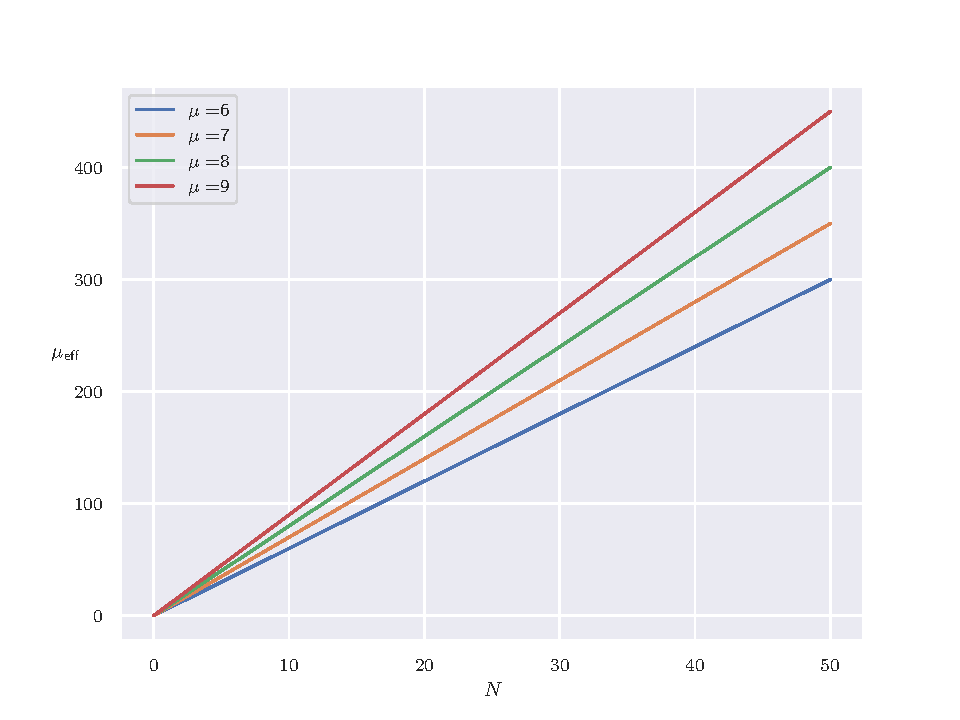
\includegraphics[width=\textwidth]{plots/mmInf_output_rate.pdf}
        \caption{Effective (aggregate) output rate in a $M/M/\infty$ system.}
        \label{fig:mmInf_output_rate}
    \end{subfigure}
    \hfill
    \begin{subfigure}[b]{0.55\textwidth}
        \centering
        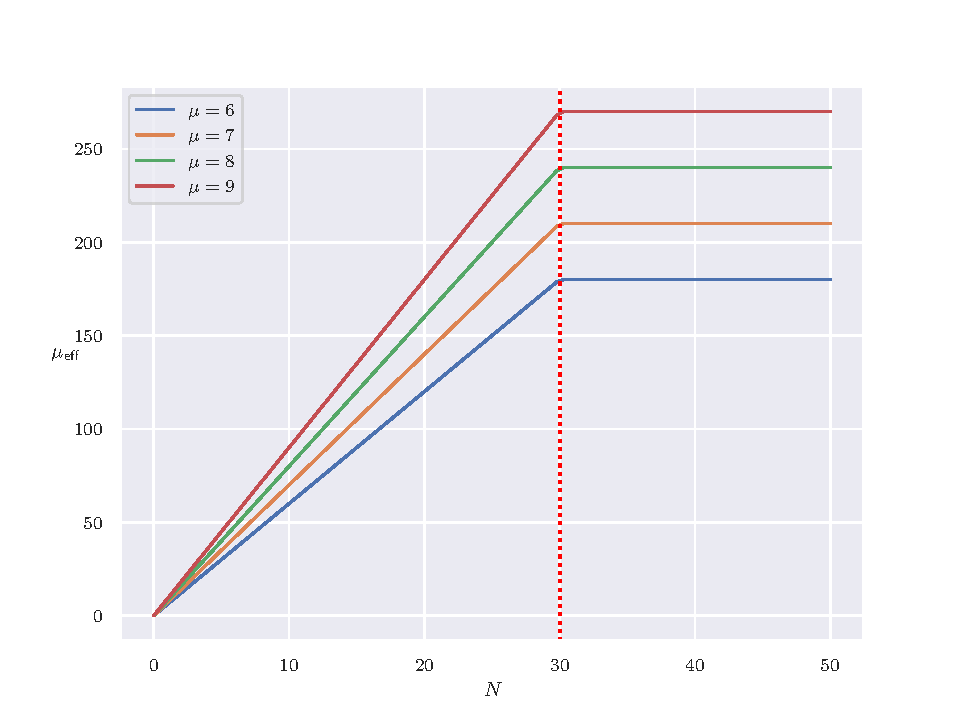
\includegraphics[width=\textwidth]{plots/mmm_output_rate.pdf}
        \caption{Effective (aggregate) output rate in a $M/M/30$ system.}
        \label{fig:mmm_output_rate}
    \end{subfigure}
    \label{fig:output_rates}
\end{figure}

\section{$M/M/m$ - $m$ Parallel servers with a queue}

\begin{figure}[ht]   
        \centering
        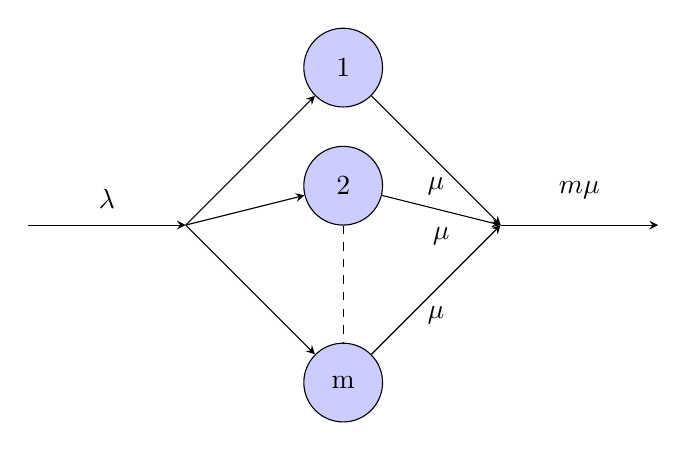
\begin{tikzpicture}[>=stealth, node distance=1.5cm, every node/.style={circle}]
    % Nodes
    \node (1) [{draw, fill=blue!20, minimum size=10mm, inner sep=0pt}]{1};
    \node (2) [{below of=1, draw, fill=blue!20, minimum size=10mm, inner sep=0pt}] {2};
    \node (m) [{below of=2, yshift=-1cm, draw, fill=blue!20, minimum size=10mm, inner sep=0pt}] {m};

    % Arrows for transitions
    \draw[->] (-2, -2) -- (1); 
    \draw[->] (-2, -2) -- (2); 
    \draw[->] (-2, -2) -- (m); 
    \draw[->] (1) -- (2, -2) node[midway, below] {$\mu$};
    \draw[->] (2) -- (2, -2) node[midway, below] {$\mu$};
    \draw[->] (m) -- (2, -2) node[midway, below] {$\mu$}; 

    % Connecting lines between nodes
    \draw[dashed] (2) -- (m);

    % Lambda arrow entering the chain
    \draw[->] (-4, -2) -- (-2, -2) node[midway, above] {$\lambda$};
    \draw[->] (2, -2) -- (4, -2) node[midway, above] {$m \mu$};
    
\end{tikzpicture}
        \caption{Flow diagram of an $M/M/m$ queue.}
    \label{fig:mmm_blk}
\end{figure}
\begin{figure}[ht]   
    \centering
    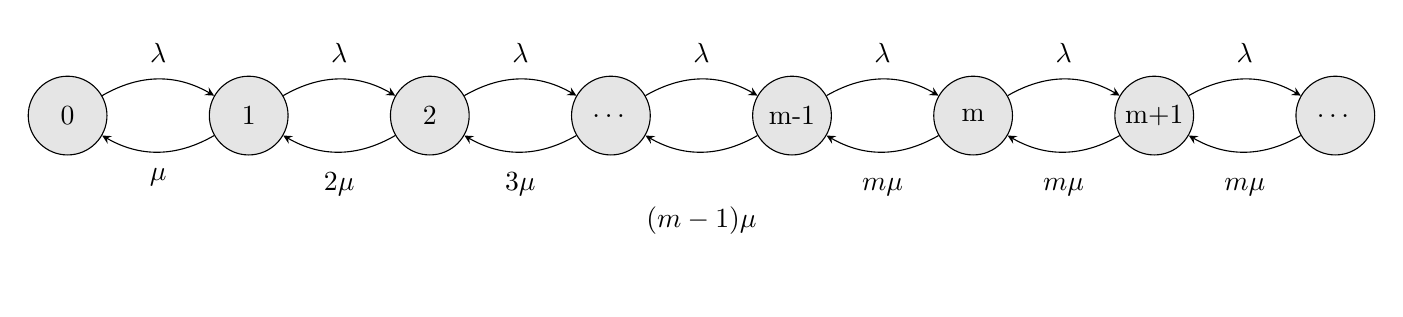
\begin{tikzpicture}[>=stealth, node distance=2.3cm, every node/.style={circle}]
    % Nodes
    \node (0) [{draw, fill=gray!20, minimum size=10mm, inner sep=0pt}] {0};
    \node (1) [{right of=0, draw, fill=gray!20, minimum size=10mm, inner sep=0pt}] {1};
    \node (2) [{right of=1, draw, fill=gray!20, minimum size=10mm, inner sep=0pt}] {2};
    \node (dots1) [{right of=2, draw, fill=gray!20, minimum size=10mm, inner sep=0pt}] {$\dots$};
    \node (m1) [{right of=dots1, draw, fill=gray!20, minimum size=10mm, inner sep=0pt}] {m-1};
    \node (m2) [{right of=m1, draw, fill=gray!20, minimum size=10mm, inner sep=0pt}] {m};
    \node (m3) [{right of=m2, draw, fill=gray!20, minimum size=10mm, inner sep=0pt}] {m+1};
    \node (dots2) [{right of=m3, draw, fill=gray!20, minimum size=10mm, inner sep=0pt}] {$\dots$};
  
  

    % Transition arrows for arrivals
    \draw[->] (0) to[bend left] node[above] {$\lambda$} (1);
    \draw[->] (1) to[bend left] node[above] {$\lambda$} (2);
    \draw[->] (2) to[bend left] node[above] {$\lambda$} (dots1);
    \draw[->] (dots1) to[bend left] node[above] {$\lambda$} (m1);
    \draw[->] (m1) to[bend left] node[above] {$\lambda$} (m2);
    \draw[->] (m2) to[bend left] node[above] {$\lambda$} (m3);
    \draw[->] (m3) to[bend left] node[above] {$\lambda$} (dots2);


    % Transition arrows for departures
    \draw[->] (1) to[bend left] node[below] {$\mu$} (0);
    \draw[->] (2) to[bend left] node[below] {$2\mu$} (1);
    \draw[->] (dots1) to[bend left] node[below] {$3\mu$} (2);
    \draw[->] (m1) to[bend left] node[below] {$(m-1)\mu$} (dots1);
    \draw[->] (m2) to[bend left] node[below] {$m \mu$} (m1);
    \draw[->] (m3) to[bend left] node[below] {$m \mu$} (m2);
    \draw[->] (dots2) to[bend left] node[below] {$m \mu$} (m3);

\end{tikzpicture}

    \caption{State transition diagram of an $M/M/m$ queue.}
\label{fig:mmm_std}
\end{figure}

Now, we make a realistic assumption and consider a model with only $m$ parallel servers. This results in a flow diagram, shown in Fig.\ref{fig:mmm_blk}, and a state transition diagram, shown in Fig.\ref{fig:mmm_std}. 

The transition rates in this case are given by:
\begin{align}
    \lambda(n) &= \lambda, && \quad n = 0, 1, 2, \ldots, \\
    \mu(n) &= n \mu, && \quad n = 1, 2, \ldots, m - 1, \\
    \mu(n) &= m \mu, && \quad n = m, m+1, m+2, \ldots.   
\end{align}

Using these rates, we get the following local balance equations,
\begin{subequations}
    \begin{align}
        p_1 &= \left( \frac{\lambda}{\mu} \right) p_0, \\
        p_2 &= \left( \frac{\lambda}{2 \mu} \right) p_1 = \left( \frac{\lambda^2}{2 \mu^2} \right) p_0, \\
        p_3 &= \left( \frac{\lambda}{3 \mu} \right) p_2 = \left( \frac{\lambda^3}{3! \mu^3} \right) p_0, \\
        \vdots \\
        p_m &= \left( \frac{\lambda}{m \mu} \right) p_{m-1} = \left( \frac{\lambda^m}{m! \mu^m} \right) p_0, \\
        p_{m+1} &= \left( \frac{\lambda}{m \mu} \right) p_m = \left( \frac{\lambda^{m+1}}{m m! \mu^{m+1}} \right) p_0, \\
        p_{m+2} &= \left( \frac{\lambda}{m \mu} \right) p_{m+1} = \left( \frac{\lambda^{m+2}}{m^2 m! \mu^{m+2}} \right) p_0, \\
        \vdots
    \end{align}    
    \label{eq:mmm_eqs}    
    Generalising, we can write in short as,
    \begin{align}
        p_n &= \frac{\lambda^n}{n! \mu^n} p_0\ &&\quad\ \text{if}\ 1 \leq n < m \\
        &= \frac{\lambda^n}{m^{n-m} m! \mu^n} p_0\ &&\quad\ \text{if}\ n \geq m.  
    \end{align}
    Using the axioms of probability,
    \begin{align}
        \sum_{n=0}^{\infty} p_n &= 1, \\
        \sum_{n=0}^{m-1} p_n + \sum_{n=m}^{\infty} p_n &= 1, \\
        p_0 \left( 1 + \sum_{n=1}^{m-1} \frac{1}{n!} \left( \frac{\lambda}{\mu} \right)^n + \sum_{n=m}^{\infty} \frac{1}{m^{n-m}} \frac{1}{m!} \left( \frac{\lambda}{\mu} \right)^n \right) &= 1, \\
        \therefore p_0 &= \left[ 1 + \sum_{n=1}^{m-1} \frac{1}{n!} \left( \frac{\lambda}{\mu} \right)^n + \sum_{n=m}^{\infty} \frac{1}{m^{n-m}} \frac{1}{m!} \left( \frac{\lambda}{\mu} \right)^n \right]^{-1}.
    \end{align}    
\end{subequations}
Thus, we can find other state probabilities in equilibrium. One important probability that we can consider is the probability of the event that there will be a queue. There will be a queue whenever, all of the $m$ servers are busy and there are arrivals.
\qs{What is the \emph{queueing} probability in an $M/M/m$ queue?}{
    \sol{
        \begin{align}
            \sP(\text{queueing}) &= \sP(n \geq m) \\
            &= \sum_{n=m}^{\infty} p_n \\
            &= \sum_{n=m}^{\infty} \frac{1}{m^{n-m}}\frac{1}{m!}(\frac{\lambda}{\mu})^n p_0 \\
            &= \frac{1}{m!}(\frac{\lambda}{\mu})^m \sum_{n=0}^{\infty}(\frac{\lambda}{m \mu})^n p_0\\
            &= \frac{1}{m!}(\frac{\lambda}{\mu})^m (\frac{1}{1 - \frac{\lambda}{m \mu}})p_0
         \end{align}
        Letting $\rho \coloneq \frac{\lambda}{m\mu}$,
        \begin{align}
            \sP(\text{queueing}) = \frac{1}{m!} (\frac{\lambda}{\mu})^m \frac{1}{1-\rho} p_0
        \end{align}
    }
}
\nt{
    Like in previous, model we can observe that the aggregate output rate of the system is proportional to the state of the system. However, now there is a limit on how much this rate can increase. See Fig.\ref{fig:mmm_output_rate}. 

    This kind of queue can provide a lot of insights in telecommunications field as this model fits many use cases in the field very well. The \emph{Queueing probability} found in the previous question represents the probability that all the servers are busy. The closed form expression of this probability is called \emph{Erlang-C formula}. Note that by substituting $\rho = 1$, we go back to the $M/M/1$ queue. Our intuition tells us that as $m$, number of servers increases, the queueing probability should go down. To verify this we have plotted this probability as a function of $m$. See Fig. 

    This metric can be used as a measure of performance of a communication system and to take decisions in the field.
}

\chapter{Summary and other models}

Finally, we have covered all the basic concepts and models that one can cover in an introductory lecture. As always, you may have a question in your mind popping up as we reach the end of this discussion: What next? Well, as we have been mentioning periodically, there are several applications of queueing theory in industrial operations, computer science, retail markets, business operations, and more. You are now ready to apply the concepts learned here and demonstrate your creativity. 

We will begin by first providing a summary of all the models discussed so far. Then, we will briefly touch upon other, more realistic models and finally conclude with a practical example where queueing theory has been applied.

\section{Summary}

We understand that reading through these notes might be exhausting. Therefore, for your quick reference, we have tabulated the results below, focusing primarily on the equilibrium state probability distributions.
\begin{center}
    \begin{tabular}{|c|c|}
        \hline
        Queueing Model & State Probability Distribution\\
        \hline
        \hline
        $M/M/1$ & 
        \begin{tabular}{@{}l@{}} 
        $p_0 = 1 - \rho$ \\ 
        $p_n = \rho^n p_0$ 
        \end{tabular} \\       
        \hline
        $M/M/1/N$ & $p_n = \big(\frac{1 - \rho}{1 - \rho ^ {N + 1}}\big) \rho ^ n\ \quad\ \ldots\ 0\leq n \leq N.$\\
        \hline
        $M/M/\infty$ & \begin{tabular}{@{}l@{}} 
            $p_n = \frac{\rho^n}{n!} e^{-\rho}$ \\
            $\therefore N \sim \text{Poisson}(\rho)$ 
            \end{tabular}\\
        \hline
        $M/M/m$ & \begin{tabular}{@{}l@{}} 
            $p_0 = \left[ 1 + \sum_{n=1}^{m-1} \frac{1}{n!} \left( \frac{\lambda}{\mu} \right)^n + \sum_{n=m}^{\infty} \frac{1}{m^{n-m}} \frac{1}{m!} \left( \frac{\lambda}{\mu} \right)^n \right]^{-1}$\\
            $p_n = \frac{\lambda^n}{n! \mu^n} p_0 \quad \text{if} \ 1 \leq n < m$\\
            $p_n = \frac{\lambda^n}{m^{n-m} m! \mu^n} p_0 \quad \text{if} \ n \geq m.$ 
        \end{tabular}\\ 
        \hline
    \end{tabular}
\end{center}

\section{Other models}
The models we have encountered so far all assumed Markovian statistics for both the arrival and departure processes. However, we need not stick to these processes. Other distributions can be used to model scenarios more appropriately.

For instance, at a bus or train ticket counter, the time required to satisfy the demands of each customer will be more or less the same. Thus, the service times can be modeled as deterministic.

\cite{RobertazziQ,myReference} also provide results for the $M/G/1$ queue. Although the method for deriving these results differs from what we have done so far, it is simple enough to follow, with some \emph{Transform Theory} involved. Those interested may refer to these sources.

More general models, such as $G/M/1$ and $G/G/1$, have analytical results derived in \cite{10.1214/aoms/1177728975,kleinrock1974queueing}.

\section{Critical Application of Queueing Theory - A case study\cite{key}}
The U.S. Military’s Air Force fleet includes 20 B-2 bombers, which require frequent maintenance. A key maintenance procedure, \emph{Low Observable} (LO), restores the special coating on the aircraft. However, maintenance scheduling and manpower distribution introduce unpredictability into the process.

The B-2's \emph{Flying Hour Program} has two main goals: maintaining operational readiness, including weapons preparedness, and ensuring wartime posture. Initially, each aircraft underwent a 200-flying hour post-flight inspection followed by \emph{heavy LO} restoration. This deterministic plan, however, resulted in poor Aircraft Availability (AA), with some B-2s completing the process in weeks, while others took up to six months.

Data analysis revealed that, on average, 4.75 B-2s were grounded for LO maintenance at any time, reducing AA to 75\%. Additionally, about 3 aircraft were grounded for other maintenance, further reducing AA to 60\%, leaving only 12 B-2s available.

To improve AA, maintenance procedures were updated. An acceptable AA range of 80-85\% (i.e., 17 B-2s) was set. Data analysis revealed that every seven days one B2 required maintenance.

We can now model this scenario using queueing theory. At any time, there is (or rather must be) a queue of, on average, at most 3 planes. Thus, we have:
\[
\bar{N} = 3.
\]
Additionally, one plane enters service every week, so the arrival rate is:
\[
\lambda = 1 \text{ per week} \quad \text{or} \quad \lambda = \frac{1}{7} \text{ per day}.
\]

By Little's Law, the average service time \(\bar{T}\) is given by:
\begin{align}
    \bar{T} &= \frac{\bar{N}}{\lambda} \\
    &= \frac{3}{\frac{1}{7}} \\
    &= 21 \text{ days}.
\end{align}

Thus, to maintain this system, the lead time for heavy LO maintenance must be 21 days. Using this estimate, the maintenance group was able to devise a schedule and routine to ensure the required AA. In this way, queueing theory played a key role in resource planning in a critical field.

\chapter{Appendix}
Only the bare minimum concepts have been covered here. I strongly advise that you go through the relevant material in \cite{pishro2014introduction}

\section{Random Processes}
\dfn{Random Process}{A random process is a collection (or a sequence) of variables usually indexed by time.
}
If the indexing variable is continuous, we refer to the process as a continuous-time random process and if the indexing variable is discrete, we call the process a discrete-time process. Thus, sampling a random process at a time instant gives a random variable. If this random variable is discrete, we call the process a discrete-valued process. Similarly, we define continuous-valued process. 

\begin{figure}
    % First subfigure: Branching Diagram
    \begin{subfigure}[b]{0.45\textwidth}
        \centering
        
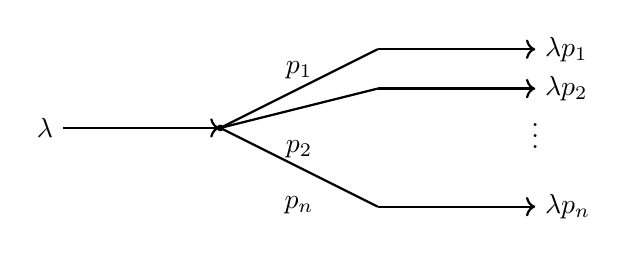
\begin{tikzpicture}
    % Draw the input arrow
    \draw[->, thick] (-2, 0) -- (-0.01, 0);
    \node[left] at (-2, 0) {$\lambda$};

    % Draw the branching point
    \filldraw (0, 0) circle (1pt);

    % Draw the branches
    \draw[thick] (0, 0) -- (2, 1);
    \draw[thick] (0, 0) -- (2, 0.5);
    \draw[thick] (0, 0) -- (2, -1);

    % Labels for probabilities
    \node[above] at (1, 0.5) {$p_1$};
    \node[above] at (1, -0.5) {$p_2$};
    \node[below] at (1, -0.75) {$p_n$};

    % Draw the output arrows for each branch
    \draw[->, thick] (2, 1) -- (4, 1);
    \draw[->, thick] (2, 0.5) -- (4, 0.5);
    \draw[->, thick] (2, -1) -- (4, -1);

    % Labels for the output flows
    \node[right] at (4, 1) {$\lambda p_1$};
    \node[right] at (4, 0.5) {$\lambda p_2$};
    \node at (4, 0) {$\vdots$};
    \node[right] at (4, -1) {$\lambda p_n$};
\end{tikzpicture}

        \caption{Splitting (Thinning of Poisson Process)}
        \label{fig:split}
    \end{subfigure}
    \hfill
    % Second subfigure: Merging Diagram
    \begin{subfigure}[b]{0.45\textwidth}
        \centering
        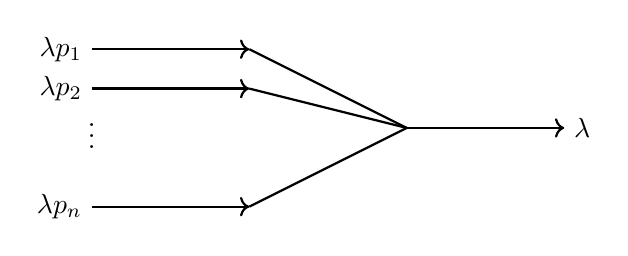
\begin{tikzpicture}
    % Draw the input arrows for each branch
    \draw[->, thick] (-4, 1.5) -- (-2, 1.5);
    \draw[->, thick] (-4, 1) -- (-2, 1);
    \draw[->, thick] (-4, -0.5) -- (-2, -0.5);

    % Labels for the input flows
    \node[left] at (-4, 1.5) {$\lambda p_1$};
    \node[left] at (-4, 1) {$\lambda p_2$};
    \node at (-4, 0.5) {$\vdots$};
    \node[left] at (-4, -0.5) {$\lambda p_n$};

    % Draw the merging point

    % Draw the branches
    \draw[thick] (-2, 1.5) -- (0, 0.5);
    \draw[thick] (-2, 1) -- (0, 0.5);
    \draw[thick] (-2, -0.5) -- (0, 0.5);

    % Draw the output arrow
    \draw[->, thick] (0, 0.5) -- (2, 0.5);
    \node[right] at (2, 0.5) {$\lambda$};
\end{tikzpicture}
        \caption{Merging of Poisson Process}
        \label{fig:merging}
    \end{subfigure}
    \label{fig:splitMerge}
\end{figure}

\dfn{Splitting (Thinning) of Possion Process}{
    Consider a parent Poisson random process with rate $\lambda$. Then, if the arrivals in this process are split into $n$ different children with probabilities $p_1, p_2, \dots, p_n$, the result is $n$ Poisson processes with rates $\lambda p_1, \lambda p_2, \dots, \lambda p_n$. Note that we must have $\sum p_i = 1$. See Fig.\ref{fig:split}.
}

\dfn{Merging of Poisson Process}{
    Let $N_1(t)$ and $N_2(t)$ be two Poisson processes with rates $\lambda_1$ and $\lambda_2$, respectively. Then, the process $N(t)$, defined as $N(t) = N_1(t) + N_2(t)$, is also a Poisson random process with rate $\lambda_1 + \lambda_2$. See Fig.\ref{fig:merging}.
}

See Fig.\ref{fig:split} and Fig.\ref{fig:merging} to understand how a process is split into multiple ones or how multiple processes are combined into a single process.

% References :
\bibliography{references}
\bibliographystyle{plain}

\end{document}
% \dfn{Limit of Sequence in }{Let be a sequence in}

% \qs{}{Is the set a closed set}
% \sol We have to take its complement and check whether that set is a open set i.e. if it is a union of open balls
% \nt{We will do topology in Normed Linear Space  (Mainly  and occasionally)using the language of Metric Space}
% \clm{Topology}{}{Topology is cool}
% \ex{Open Set and Close Set}{}